\chapter{\label{ch:4-ams}The American monsoon system in UKESM1 and HadGEM3}


This chapter evaluates the representation of the AMS in the contributions to CMIP6 from UKESM1 and HadGEM3. The pre-industrial control, historical and AMIP experiments described in section \ref{sq:modeldata} are evaluated for their large and regional-scale biases, as well as their representation of key teleconnection patterns.
The simulations show a good representation of the seasonal cycle of temperature, although the historical experiments overestimate the observed summer temperature in the Amazon, Mexico and Central America by more than 1.5 K.
The seasonal cycle of rainfall and general characteristics of the North American Monsoon in all the simulations agree well with observations, suggesting  a notable improvement from previous versions of the HadGEM model.
 The models reasonably simulate the bimodal regime of precipitation in southern Mexico, Central America and the Caribbean known as the midsummer drought, although  with a stronger than observed difference between the two peaks of precipitation and the dry period. 
Austral summer biases in the modelled Atlantic Intertropical Convergence Zone (ITCZ), cloud cover and regional temperature patterns are noteworthy and influence the simulated regional rainfall in the South American Monsoon.
These biases are associated with an overestimation of precipitation in southeastern Brazil and an underestimation of precipitation in the Amazon which are greatly reduced in the AMIP simulations, highlighting that an accurate simulation of the Atlantic SSTs is key for representing precipitation in the South American Monsoon.  
  El Ni\~no Southern Oscillation (ENSO) teleconnections, of precipitation and temperature, to the AMS are reasonably simulated by all the experiments. 
The precipitation responses to the positive and negative phase of ENSO in subtropical America are linear in both pre-industrial and historical experiments, in contrast to observations.
  Overall, the biases in UKESM1 and the low resolution configuration of GC3 are very similar for precipitation, ITCZs and the Walker circulation, i.e., the inclusion of  Earth System processes appears to make no significant difference for the representation of the AMS rainfall. 
In contrast, the medium resolution HadGEM3 N216 simulation outperforms the low-resolution simulations due to improved SSTs and circulation.


 % Model assessment and validation is also important for this purpose as this process 

\section{Introduction}

The response of regional monsoons to greenhouse forcing remains an open question \citep{zhou2016,pascale2019} because the observational record is too short to exhibit significant trends but also because biases in GCMs increase uncertainty in future model projections.
Although the thermodynamical response to greenhouse forcing in tropics seems to be relatively well constrained, the dynamical response is less clear \citep{shepherd2014}. The American Monsoon System (AMS), as most monsoon regions is shaped by regional dynamical features which makes the dynamical biases particularly relevant when understanding the precipitation response to forcing in a monsoon region. % for monsoons. 

In spite of current recognition as a monsoon, the AMS has received less attention by the modelling community compared to the Asian or African monsoons. 
The assessment of climate models in monsoon regions is key to understand current and future changes to the water cycle in tropics. However, in the AMS, model assessments are usually only done in a handful of studies per CMIP phase.  These studies only provide a wide view of the biases of each generation of models while usually highlighting which biases have improved and which biases remain from previous model generations \citep[see e.g.][]{geil2013,ryu2014}. However, a deeper evaluation of individual models can be used to provide better insight into the processes associated with climatological biases in the large-scale circulation and ultimately better understand the causes for the model biases in AMS rainfall. 

For example, in the South American Monsoon, CMIP5 models improved from CMIP3 in the simulated distribution of precipitation during monsoon maturity and exhibited an improved seasonal cycle \citep{jones2013,yin2013}. However, biases in the South American Monsoon, e.g., the underestimation of rainfall in the central Amazon, have persisted from the first generation of GCMs up until CMIP5 \citep{li2006,yin2013}. The geographic distribution of rainfall during  austral fall and several characteristics of the South Atlantic Convergence Zone are also poorly represented in CMIP5. However, these studies provided little evidence as for the reasons for the improvements or the remaining biases in the models. 
A clear motivation to evaluate models in the South American Monsoon is that the accurate simulation of the geographic distribution and seasonality of rainfall in the Amazon rainforest is a relevant issue due to the impact of the rainforest on climate and society \citep[e.g.][]{li2006,Malhi20610,yin2013} and thus more research on the representation of the South American Monsoon is warranted.

Climate research in recent decades has aimed to reduce uncertainty in climate projections by improving GCMs, but different approaches taken by modelling centres are seemingly disconnected \citep{jakob2014}. One approach is to reduce horizontal grid spacing down to km resolution to rely less on parametrizations and more on physical laws to represent clouds and convection \citep{palmer2019}. A second approach aims to include new explicit representation of Earth System processes to better characterise complex land-atmosphere-ocean biogeochemical cycles that may provide a better constraint on large-scale aspects of the climate such as climate sensitivity, a parameter that depends on the carbon cycle \citep{marotzke2017,sellar2019,andrews2019}. Finally, recent modelling centres have chosen to include  stochastic  parametrisations of sub-grid processes since this approach has improved seasonal forecasts and may therefore improve climate projections \citep{palmer2019st}. 

Model validation and assessment is important to analyse the effect of new parametrisations and to highlight missing processes but also evaluate which route provides the more substantial model improvement, stochastic parametrisations, increased resolution or Earth Sytem processes.
The focus of this chapter is then to evaluate the CMIP6 experiments from HadGEM3 GC3.1 (GC3) and UKESM1 in the AMS. In this chapter and remainder of the thesis, the AMS is considered to be composed of the North and South American monsoon systems, while also including the Midsummer drought region of southern Mexico and Central America as part of the AMS \citep[as in e.g.][]{vera2006,pascale2019}.

The remainder of this chapter is organised as follows. The following section described the data and methods used in this chapter. Section  \ref{sq:clim} compares modelled and observed climatological temperature, sea-level pressure and low-level wind fields,  whereas section \ref{sq:itcz} analyses the Pacific and Atlantic ITCZs. Section \ref{sq:precip} analyses the spatial and temporal characteristics of rainfall and convection in the AMS while section \ref{sq:enso1} documents the simulated teleconnections of ENSO. A summary and discussion of the results is provided at the end of the chapter.

\section{Methods and data} 

The model assessment of this chapter will use a range of experiments from the MOHC. The piControl experiments from GC3 and GC3 N216 are used to evaluate the role of resolution whereas the historical experiments from UKESM1 and GC3 are used to evaluate model skill in reproducing the observed period whereas the AMIP experiment from GC3 is used to highlight the role of SST biases. The historical experiment data is used only in the 1970-2014 period whereas the whole pre-industrial and AMIP available data is used. 
All the datasets used in this chapter are thoroughly described in chapter \ref{ch:3-methods} but in summary in this chapter, the surface or near-surface air temperature data is taken from the CRU4 dataset and ERA5, whereas precipitation is used from the different datasets described in the previous chapter. The dynamical features such as wind speed and vertical velocity are taken from ERA5.

The climate indices of ENSO and the QBO used in this chapter were obtained by the following process. 
For ENSO, the deseasonalized and detrended time-series of the area-averaged SSTs (EN3.4 region [190-240$^\circ$W,5$^\circ$S-5$^\circ$N]) is used as an index to composite months into positive, negative and neutral phases. 
A month is determined to be in the positive, El Niño, phase when the index is higher than +0.65 K and a negative phase, La Niña, when the index is more negative than -0.65 K. A neutral month is found where the magnitude of the index is smaller than 0.5 K.  Other indices, including the use of a 5-month running mean \citep{trenberth1998}, were tested without significantly changing the results.   Previous studies \citep[e.g.][]{menary2018,kuhlbrodt2018}  showed that the MOHC models reasonably simulate several characteristics of ENSO such as the period and SST patterns.

Similarly, for the QBO, the deseasonalized and detrended time-series of the equatorially averaged [10$^\circ$S-10$^\circ$N] zonal-mean zonal wind at the 70 hPa level is used as the QBO index for both reanalysis and model data. The westerly phase of the QBO (QBOw) is determined when the index is greater than 2 m s$^{-1}$ and the easterly phase (QBOe) when the index is less than -2 m s$^{-1}$. 

%Therefore, this chapter compares the effect of increased horizontal resolution and Earth System processes  on the representation of the AMS in a climate model. In this chapter, in addition to the historical experiments which are more suitable for model assessment, both the pre-industrial control and atmosphere-only experiments are also used. 
%For example, HadGEM3 was run at two horizontal resolutions for CMIP6, and UKESM1 can also be directly compared to 

% 
%The validation of climate models is important for multiple purposes, for example, to evaluate the effect of new  % and the potential use of the models to answer outstanding questions of the monsoon long-term variability and teleconnections. 
%A principal use of climate models is their role in climate projections that aim to roughly predict the effect of a given forcing, i.e., greenhouse warming, over global and regional climate. 
%The robustness and confidence in model projections depends on the results from model assesment and validations.



%In this chapter, two resolutions of the climate model HadGEM3 are compared against UKESM1, which has the same dynamical core and physical parametrisations, but with additional components of the Earth System (see section \ref{sq:modeldata}). 




%Overall, very few studies have analysed the relative roles of large-scale biases for monsoon representation or the links between features such as the ITCZ or the Walker circulation and the AMS, which may be particularly important when understanding projected responses to forcing \citep{zhou2016,wang2017}. }

 
%C
% The next efforts to improve climate models include increased horizontal resolution, better parameterisations and/or the addition of processes in new models known as Earth System models \citep{eyring2016}.
 %The new phase of the CMIP project will include a range of new submissions which will include models with higher resolution and more Earth System models \citep{eyring2016}. A comparison and evaluation of simulations with increased horizontal resolution and Earth System models may suggest where modelling efforts are resulting in significant improvements in model representation of monsoons.

%
%\section{Climatological features}\label{sq:clim}


\section{Climatological temperature and low-level wind biases} \label{sq:clim}

\begin{figure}[t!]
\centering
 %\noindent
 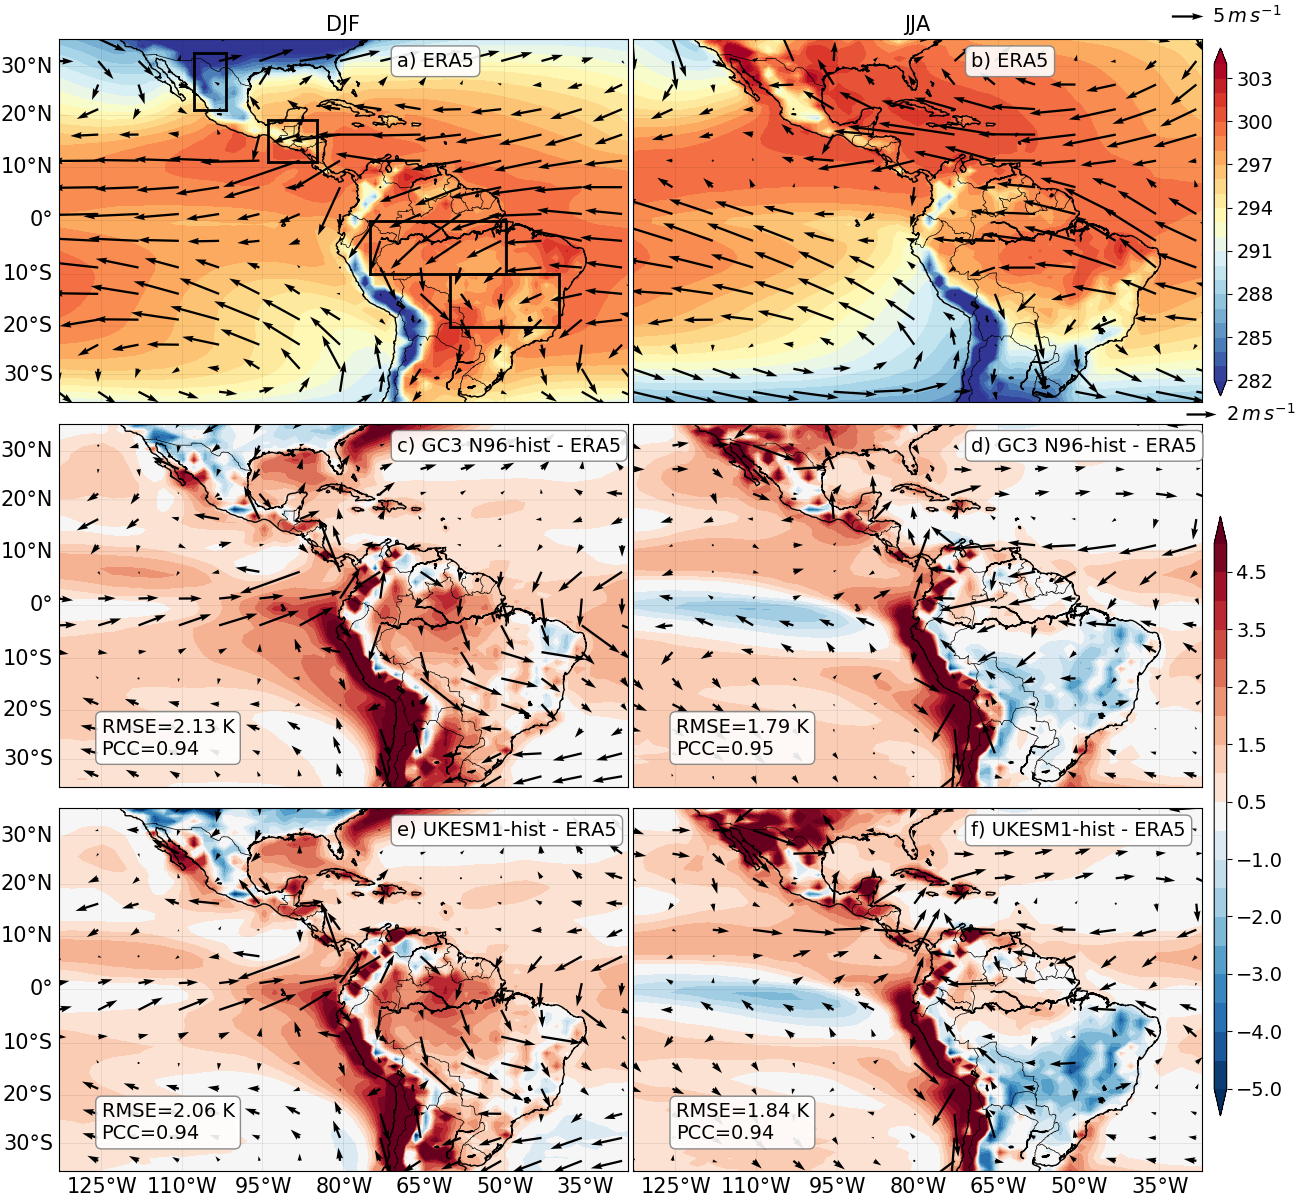
\includegraphics[width=\linewidth]{figures/fig1p2_f1a.png}
\caption{ (a, b) Temperature (color-contours in K) and wind speed (vectors) at 850 hPa DJF and JJA climatogies in ERA5. The biases are shown as the differences between the ensemble mean from the historical experiment of (c, d) GC3 and  (e, f) UKESM1 and ERA5.
The climatogies and biases are shown for (a, c, e) boreal winter (DJF) and (b, d, f) boreal summer (JJA). Only differences statistically significant to the 95\% level are shown, according to a Welch t-test for each field. The key for the size of the wind vectors is shown in the top right corner of panels b) and d). The root-mean square error (RMSE) and pattern correlation coefficient (PCC) are shown on the bottom left of c-f.}
\label{fig:1}
\end{figure}

This section evaluates the simulated climatological temperature and low-level wind structure in the AMS region.
The climatological representation of the near-surface air temperature and low-level winds in the models is compared to ERA5 in Figures \ref{fig:1} and \ref{fig:1b}, the climatology of DJF and JJA of ERA5 is shown in Figure \ref{fig:1}a, b.
The biases of the historical experiments, computed as the differences between the model and observed fields, are shown in Figures \ref{fig:1}c, d) for GC3-hist and e, f) for UKESM1-hist.
 Only statistically significant differences are shown, according to a Welch t-test \citep{wilks2011}, which accounts for the difference in sample size and variance between model and observations/reanalysis data. The significance for simulations with multiple ensemble members is estimated first for each ensemble member and then combined into a single probability or p-value using Fisher's method \citep{fisher1992statistical}. Pattern correlations and root-mean square error (RMSE) are shown in Figures \ref{fig:1}c-f and in Table \ref{tab:s1}.
 

\begin{table}[t!]
\small
\caption{\small Root-mean square error (RMSE) and pattern correlation coefficients (PCC) for each season and each model experiment. Near surface air temperature ($t2m$), wind components ($u$ and $v$) and mean-sea level pressure ($mslp$) are assessed against ERA-5 and precipitation ($pr$) against TRMM.}
\begin{tabular}{p{1.05cm}|p{2.25cm}|p{1.10cm}p{1.10cm}p{1.10cm}p{1.10cm}p{1.10cm}p{0.9cm}p{1.05cm}p{1.05cm}} \label{tab:s1}
  \textit{Variable}                  & \textit{Experiment}  & DJF RMSE & DJF PCC & MAM RMSE & MAM PCC & JJA RMSE & JJA PCC &  SON RMSE & SON PCC \\ \hline \hline
t2m & GC3 N96 & 1.28 & 0.98 & 1.3 & 0.96 & 1.38 & 0.96 & 1.31 & 0.96 \\
t2m & GC3 N216 & 1.05 & 0.99 & 1.07 & 0.98 & 1.02 & 0.98 & 0.98 & 0.98 \\
t2m & GC3 Hist & 2.06 & 0.94 & 1.75 & 0.93 & 1.73 & 0.94 & 2.05 & 0.92 \\
t2m & UKESM-hist & 2.03 & 0.94 & 1.77 & 0.93 & 1.8 & 0.94 & 2.0 & 0.93 \\
t2m & GC3 AMIP & 1.17 & 0.98 & 1.12 & 0.97 & 1.2 & 0.97 & 1.2 & 0.97 \\
u & GC3 N96 & 0.78 & 0.99 & 0.59 & 0.99 & 0.9 & 0.98 & 0.87 & 0.98 \\
u & GC3 N216 & 0.78 & 0.99 & 0.59 & 0.99 & 0.9 & 0.98 & 0.87 & 0.98 \\
u & GC3 Hist & 1.02 & 0.98 & 1.04 & 0.97 & 0.92 & 0.98 & 0.84 & 0.98 \\
u & UKESM-hist & 1.04 & 0.98 & 1.01 & 0.97 & 0.91 & 0.98 & 0.82 & 0.98 \\
u & GC3 AMIP & 0.96 & 0.98 & 0.77 & 0.99 & 1.18 & 0.97 & 1.09 & 0.96 \\
v & GC3 N96 & 0.75 & 0.93 & 0.66 & 0.93 & 0.65 & 0.95 & 0.59 & 0.94 \\
v & GC3 N216 & 0.6 & 0.96 & 0.5 & 0.95 & 0.57 & 0.96 & 0.54 & 0.94 \\
v & GC3 Hist & 0.76 & 0.94 & 0.72 & 0.92 & 0.66 & 0.95 & 0.59 & 0.94 \\
v & UKESM-hist & 0.75 & 0.93 & 0.69 & 0.92 & 0.65 & 0.95 & 0.6 & 0.93 \\
v & GC3 AMIP & 0.67 & 0.95 & 0.52 & 0.95 & 0.68 & 0.94 & 0.61 & 0.93 \\
mslp & GC3 N96 & 1.33 & 0.96 & 1.03 & 0.97 & 1.15 & 0.96 & 0.95 & 0.97 \\
mslp & GC3 N216 & 1.11 & 0.97 & 0.9 & 0.97 & 1.1 & 0.96 & 0.89 & 0.97 \\
mslp & GC3 Hist & 1.31 & 0.97 & 1.12 & 0.96 & 1.08 & 0.96 & 0.94 & 0.97 \\
mslp & UKESM-hist & 1.4 & 0.97 & 1.15 & 0.96 & 1.14 & 0.95 & 0.99 & 0.97 \\
mslp & GC3 AMIP & 1.15 & 0.97 & 0.87 & 0.97 & 1.09 & 0.96 & 0.93 & 0.97 \\
pr & GC3 N96 & 2.02 & 0.79 & 2.24 & 0.71 & 1.62 & 0.9 & 1.69 & 0.86 \\
pr & GC3 N216 & 1.58 & 0.88 & 1.72 & 0.85 & 1.4 & 0.93 & 1.57 & 0.89 \\
pr & GC3 Hist & 2.05 & 0.78 & 2.49 & 0.64 & 1.69 & 0.88 & 1.69 & 0.86 \\
pr & UKESM-hist & 1.96 & 0.8 & 2.39 & 0.66 & 1.71 & 0.88 & 1.62 & 0.87 \\
pr & GC3 AMIP & 1.42 & 0.9 & 1.61 & 0.88 & 1.95 & 0.88 & 1.8 & 0.88 \\
\end{tabular}
\end{table}  

\begin{figure}[t!]
\centering
 %\noindent
 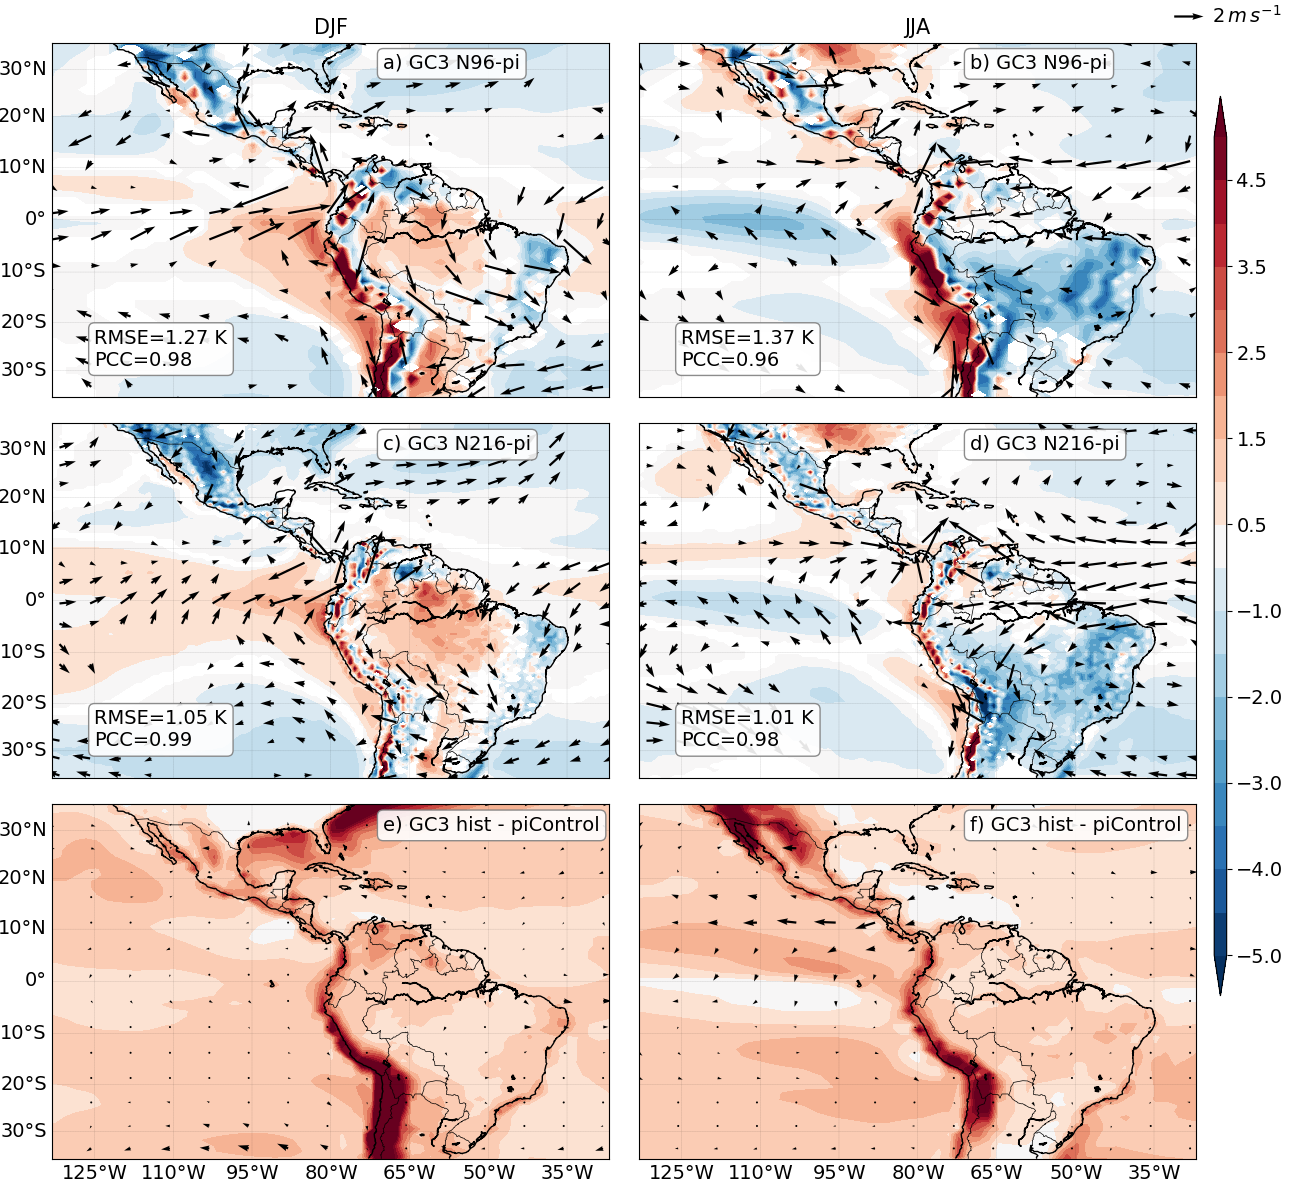
\includegraphics[width=\linewidth]{figures/fig1p2_f1b.png}
\caption{ As in Figure \ref{fig:1}, but showing the differences between the piControl simulations of (a, b) GC3 N96-pi and (c, d) GC3 N216-pi, and ERA5. (e, f) show the statistically significant differences between the historical (1979-2014) and piControl experiments of GC3.  The RMSE and PCC are shown on the bottom left of a-d.}
\label{fig:1b}
\end{figure}

 During DJF, the simulations show a colder-than-observed sub-tropical North America and a warm bias over the Amazon ($\approx +3.5$ K).
 The west coast of South America also shows a significant warm bias ($>+4$ K) in the historical simulations.
 The simulated circulation in austral summer in South America has a significant bias in the easterly flow coming from the equatorial and subtropical Atlantic.
 The low-level wind biases suggest a weaker easterly flow from the Atlantic into southeastern Brazil but also a strong southward flow from northern to southern South America.
  The South America Low-Level Jet, i.e., the low-level northwesterly flow in Bolivia, observed in Figure 1a, is stronger in the simulations.
   This stronger than observed jet is suggestive of a stronger moisture transport to the La Plata Basin, which has been associated with a drying of the Amazon and positive precipitation anomalies at the exit region of the jet \citep{marengo2012,jones2017}.
  % \citep


In turn, in boreal summer (Figures \ref{fig:1}d, f), positive temperature biases are observed in southwestern North America ($>+3.5 $ K), which are higher in UKESM1-hist than in GC3-hist.
 The easterly flow west of Central America has a negative bias in UKESM1 suggesting a weaker flow that crosses from the Caribbean Sea into the East Pacific Ocean.
 %Both models show an anticyclonic anomaly in the region of the North Atlantic Subtropical High.
 Also in JJA, the simulated East Pacific surface temperatures are colder than observed for both historical experiments.      The inclusion of Earth System processes appears to make no  improvement on the low-level circulation biases. 

The piControl simulations (Figures \ref{fig:1b}a-d) have some similar biases to the historical simulations.
 In DJF, the piControl simulations show a similar but smaller positive bias in the Amazon than the historical experiments, as well as a similar bias in the circulation in South America, with the smallest biases in GC3 N216 piControl.
 In JJA, the piControl simulations do not show the positive temperature bias in northwestern North America. However, the bias in the zonal wind over the easternmost Pacific is present in both piControl and historical simulations.
 
 Figures \ref{fig:1b}e, f show the difference between the historical and piControl experiment of GC3, illustrating the response to historical forcing in GC3.
 The temperature response in austral summer in South America is observed as 1.5 K whereas in JJA in North America temperatures were 4 K higher in the historical experiment than in the piControl.
 A very similar temperature pattern response to historical forcing was observed for UKESM1 (not shown) although of slightly different magnitude. The only significant difference in low-level winds, as a response to historical forcing, are the easterlies in the East Pacific Ocean during JJA, which are stronger in the historical simulation. %hereas the rest of the low-level wind

%The SLP and wind biases show that during boreal winter, a lower-than-observed SLP in southern South America of -2 hPa, is associated with a northwesterly wind anomaly into southeastern Brazil. This anomalous circulation is weaker in GC3.1 n216 than in the other two simulations.

\begin{figure}[t!]
\centering
 %\noindent
 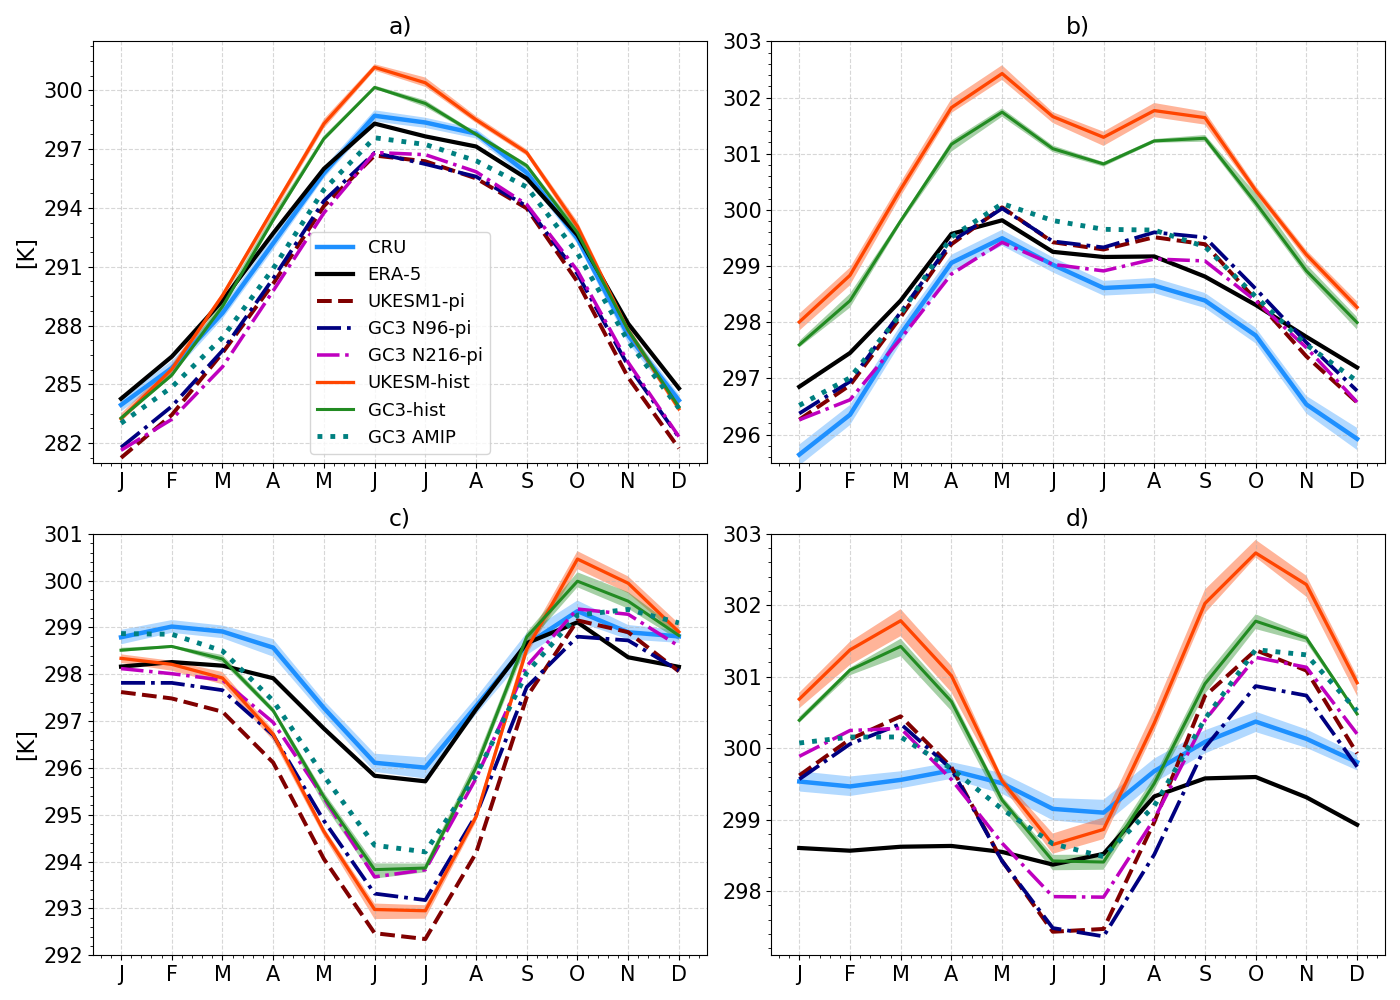
\includegraphics[width=\linewidth]{figures/p2fig2_v3.png}
\caption{ Monthly-mean temperature in the (a) North American Monsoon [19-35$^\circ$N,110-103$^\circ$W], (b) the Midsummer drought [11-19$^\circ$N,95-85$^\circ$W] (c) Eastern Brazil [20-10$^\circ$S,60-40$^\circ$W] and (d) the Amazon basin [-10-0$^\circ$S,75-50$^\circ$W] regions. The shadings for the CRU dataset represents the observational uncertainties and for the historical simulations the shading is the ensemble spread. The regions for this plot are shown in Figure \ref{fig:1}a. }
\label{fig:2}
\end{figure}

The seasonal cycle of temperature in key regions (depicted in Figure \ref{fig:1}a) of the AMS is shown in Figure \ref{fig:2}, comparing the simulations to ERA5 and the CRU4 dataset.
The temperature in the North American Monsoon region ranges from the boreal winter mean temperature of 12$^\circ$C to a maximum in June close to 27$^\circ$C.
Although the piControl simulated temperatures are colder than observed throughout the year, the models reasonably reproduce the seasonal cycle, which may be relevant for the simulated monsoon onset timing and strength \citep{turrent2009}. The historical experiments notably show a colder than observed winter and a warmer than observed summer.

The piControl simulations show a colder-than-observed winter in southern Mexico and northern Central America. The historical experiments show a warming signal, when compared to the piControl simulations, of about 1.5 K in winter and 2 K in the summer in this region. In spite of these biases, all the experiments follow closely the seasonal cycle in North and Central America.

However, the seasonal cycle in South American regions (Figures \ref{fig:2} c, d) of southeastern Brazil and the central Amazon shows notable temperature biases.
The simulations show a stronger than observed seasonal cycle, especially the historical experiments. For example, the modelled temperature difference between late austral winter and spring was $\approx$4 K whereas the observed temperature varies by less than 1 K in the same period. The models show a warm bias in the Amazon region (Fig. \ref{fig:2} d) which peaks in austral spring (SON), during the development of the monsoon \citep{marengo2012}.
In southeastern Brazil, the seasonal cycle is reasonably well reproduced but with a significant cold bias throughout the year which maximizes during austral winter (JJA), as models (e.g. UKESM1) simulate  a temperature 4 K lower than observed.
In all panels of Figure \ref{fig:2}, the historical experiments show a significant warming signal as a response to historical forcing, which is generally stronger in UKESM1 than in GC3. 

\section{The Atlantic and Pacific ITCZs and the SACZ}\label{sq:itcz}



The AMS is intertwined with the seasonal migration of the East Pacific and Atlantic ITCZ as the ITCZ largely determines regions of ascending and descending motions, moisture transport and the hemispheric energy balance \citep{oueslati2013,li2014,zhou2016,cai2019pantropical}. In particular, the North American monsoon and MSD are mostly influenced by the East Pacific ITCZ whereas the South American monsoon is affected by the strength and position of the Atlantic ITCZ \citep{yoon2010atlantic,marengo2012}. 
%This section validates the modelled ITCZs and Walker circulation.
%The ITCZ position is largely a result of atmospheric and oceanic energy transport \citep{schneider2014}, which are difficult to represent in GCMs and led to the double ITCZ problem \citep{li2014}.


Figure \ref{fig:3} shows the observed and modelled climatological rainfall and the ITCZ climatological positions. Three simulations are shown: the ensemble-mean UKESM1-historical, the ensemble mean GC3 AMIP and GC3 N216-pi.
Other simulations are not shown as all the coupled low resolution simulations showed very similar precipitation and ITCZ characteristics whereas the AMIP and medium-resolution experiments showed notable differences.

\begin{figure}[t!]
\centering
 %\noindent
 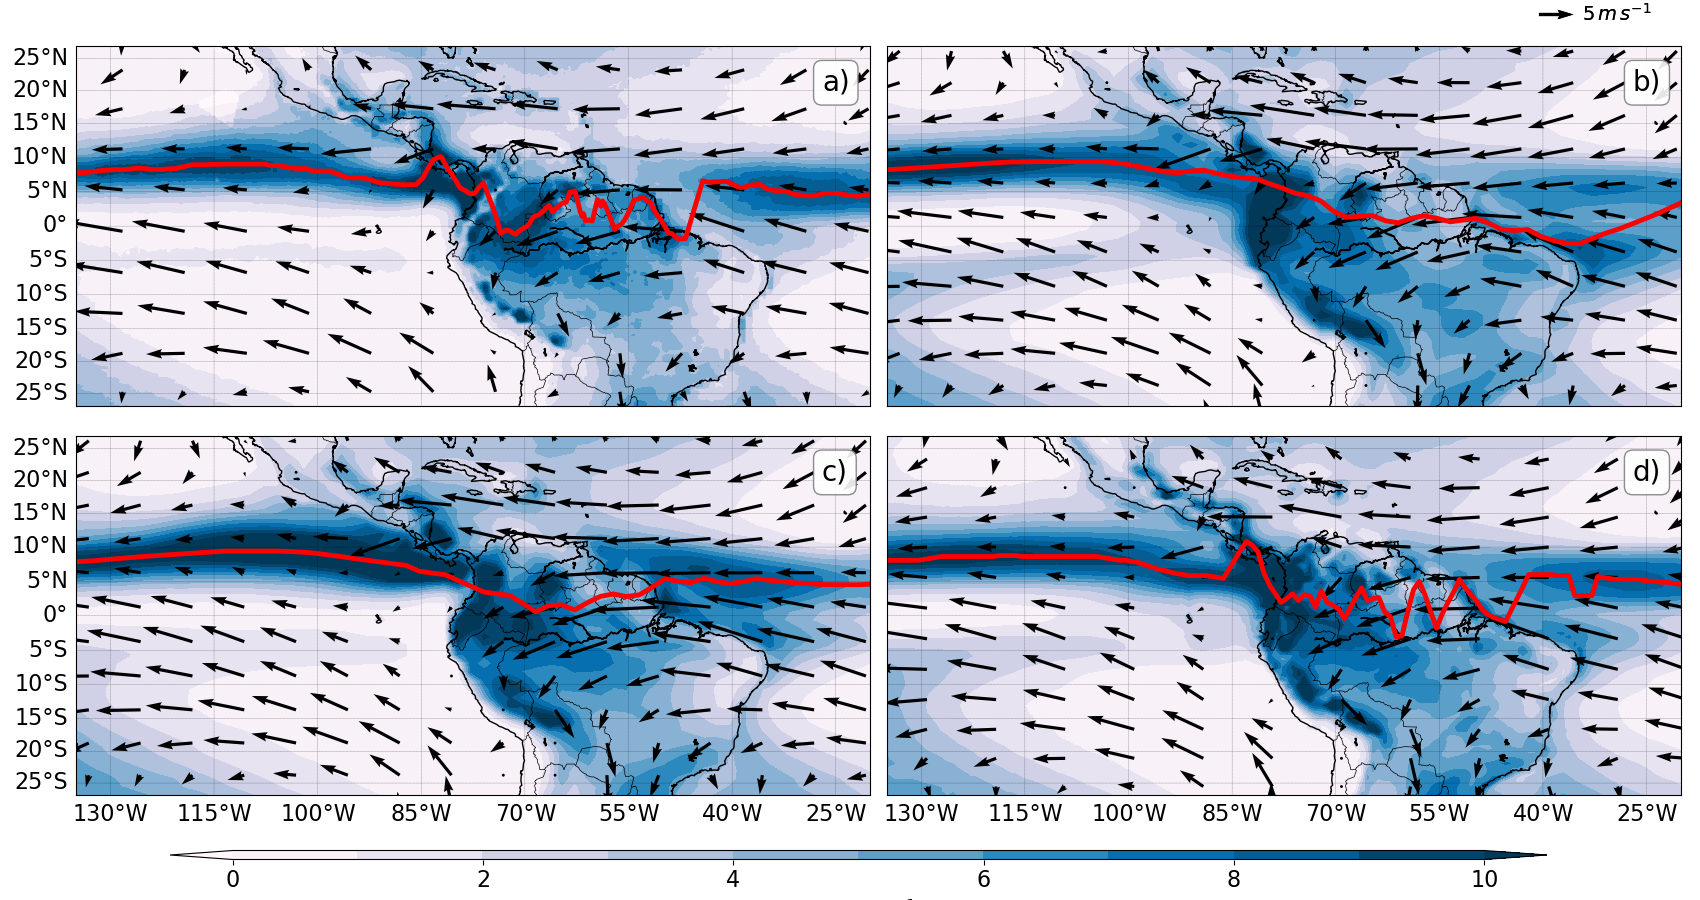
\includegraphics[width=\linewidth]{figures/itcz_clim_d.png}
\caption{ Climatological rainfall [mm day$^{-1}$] and low-level wind speed (850-hPa) in (a) TRMM and ERA-5, (b) the ensemble-mean UKESM-historical, (c) GC3-amip and (d) GC3 N216-pi. The red line highlights the maximum rainfall for each longitude as a proxy for the position of the ITCZ.  }
\label{fig:3}
\end{figure}

The climatological ITCZ in TRMM (Figure \ref{fig:3}a) is found, on average, at 8$^\circ$N in the East Pacific and at 6$^\circ$N in the Atlantic.
All the simulations reasonably represent the climatological position of the East Pacific (EP) ITCZ; however, the modelled Atlantic ITCZ near the coast of Brazil is found south of the equator at 3$^\circ$S in the coupled model simulations.
The location of the ITCZ in GC3 N216-pi and the spatial distribution of rainfall is more consistent with TRMM dataset than the rest of experiments.
Rainfall near the Amazon river mouth is significantly larger in the low resolution simulations than in the TRMM dataset. 
 However, the GC3 AMIP shows the best agreement with TRMM in ITCZ position and rainfall distribution. 

\begin{figure}[t!]
\centering
 %\noindent
 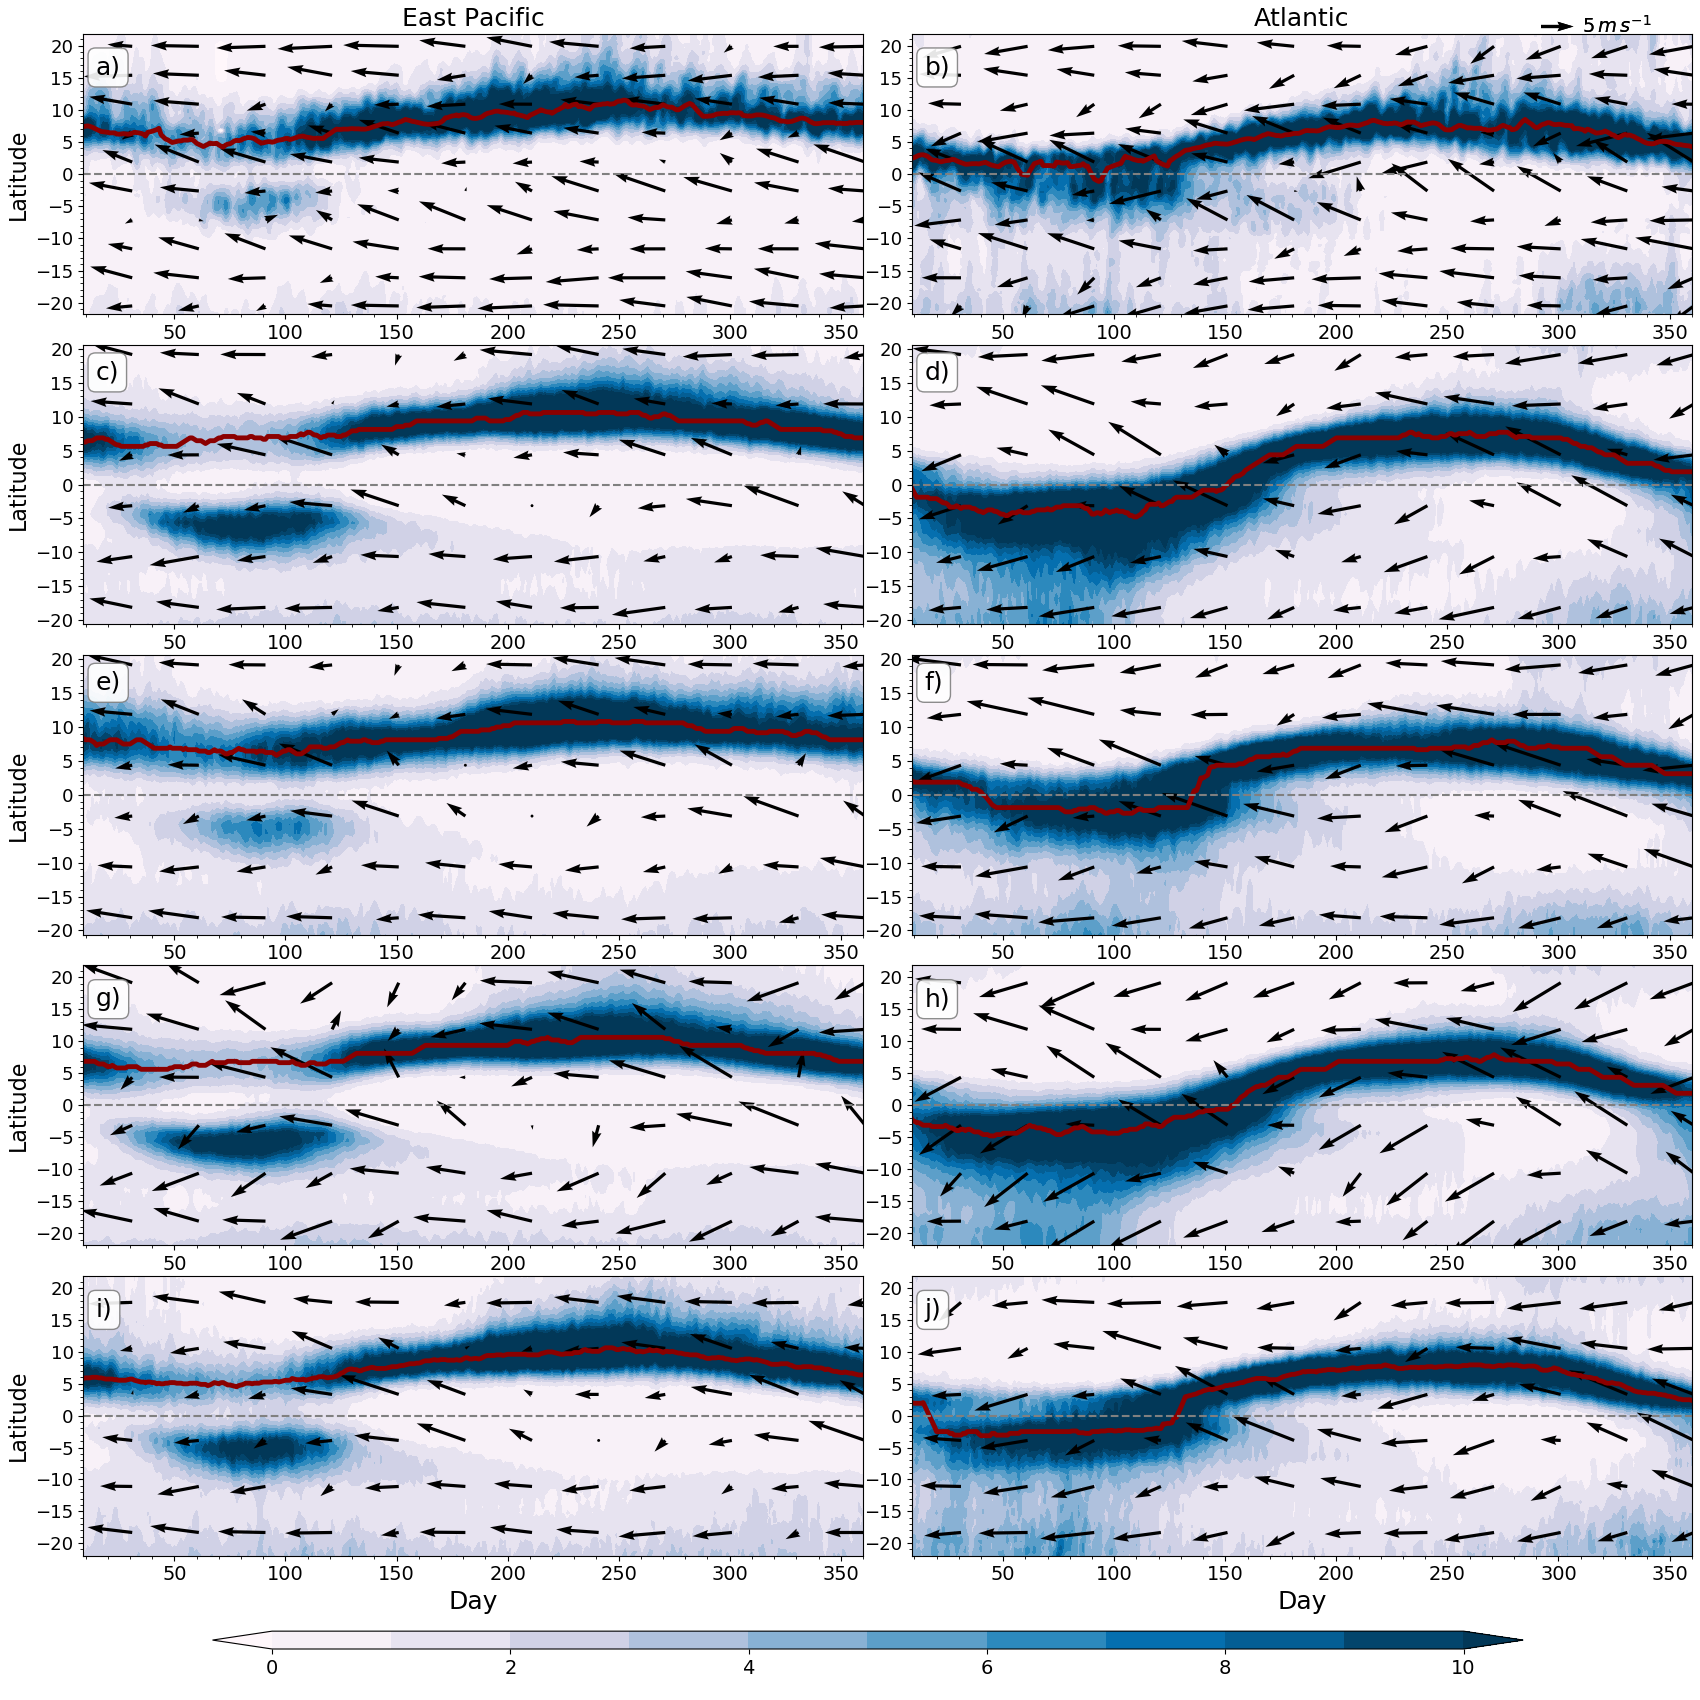
\includegraphics[width=\linewidth]{figures/fig3_p2_v3.png}
\caption{ Time-Latitude plot of daily mean rainfall (colour contours) and low-level wind speed (850 hPa) longitudinally averaged over the (a, c, e, g) East Pacific [150$^\circ$W-100$^\circ$W] and (b, d, f, h) Atlantic [40$^\circ$W-20$^\circ$W] Oceans. (a, b) show rainfall from TRMM and winds from ERA-5, (c, d) the ensemble-mean UKESM-historical, (e, f) GC3 AMIP, (g, h) N96-pi and (i, j) GC3 N216-pi. The red solid line shows the ITCZ as the latitude of maximum precipitation.  }
\label{fig:4}
\end{figure}


The seasonal cycle of the ITCZ location, precipitation rates and low-level winds in both basins are shown in Figure \ref{fig:4}, for TRMM, UKESM1-hist, GC3 AMIP, GC3 N96-pi and GC3 N216-pi.   %, two piControl and one historical simulations.
The EP ITCZ in observations (Fig. \ref{fig:4}a) migrates southwards during the first days of the year and is weakest and at its southernmost position at 5$^\circ$N around day 100 (mid-April).  
During boreal spring, the EP ITCZ migrates northward reaching a peak latitude and maximum rainfall at 10$^\circ$N by day 250, or early September. The EP ITCZ during boreal winter is weaker than during the rest of the seasons.
The low-level winds are predominantly easterly, which are stronger away from the ITCZ and weaker and convergent near the ITCZ position.
The position and seasonal migration of the EP ITCZ is reasonably well represented in the four simulations (Figs. \ref{fig:4}c, e, g, i), but a noticeable bias in precipitation is observed in  boreal winter south of the equator in the coupled simulations. The modelled  low-level winds in the coupled simulations show significant biases near the ITCZ.
These wind biases are observed as stronger wind vectors converging toward the ITCZ during boreal summer and spring and stronger wind vectors diverging away from the equator during boreal winter. 

The observed Atlantic ITCZ (Figure \ref{fig:4}b) has a similar seasonal cycle to the EP ITCZ.
The Atlantic ITCZ is close to 4$^\circ$N at day 1 and migrates southwards at the start of the year reaching  its southernmost position at 0$^\circ$ at the end of March.
During boreal spring, the Atlantic ITCZ migrates north, reaching 8$^\circ$N at the start of boreal summer. In contrast to the EP ITCZ, the maximum rainfall in the Atlantic ITCZ does not weaken during any season. 
The boreal winter position of the modelled ITCZ is displaced south with respect to the observations.
The simulated ITCZ  crosses south of the equator during boreal winter, as high rainfall rates above 12 mm day$^{-1}$ covering the 10S-0 region.
After boreal spring, the modelled ITCZ crosses back north of the equator and matches the observed ITCZ reasonably well for boreal summer and fall.
Low-level wind vectors near the Atlantic ITCZ (Figures \ref{fig:4}f and h) suggest a simulated southerly bias north of the equator and a stronger northerly flow south of 10$^\circ$S.




The biases in the Atlantic ITCZ can also be observed in the overturning circulation (not shown) and the associated Walker circulation as significant negative $\omega$ and $q$ biases just north and south of equatorial South America indicative of weaker convective activity. The simulated Atlantic Ocean has a biased negative $\omega$ (more ascent) south of the equator and a positive $\omega$ bias (less ascent) north of the equator in the low resolution simulations.
These biases in the Atlantic ITCZ and overturning circulations described above were found to be of similar magnitude in all the coupled model simulations run at lower resolution, both historical and piControl experiments,   however, these biases improved in the medium resolution GC3 N216-pi and in the AMIP simulations (Figures \ref{fig:4}f, j). 

\begin{figure}[t!]
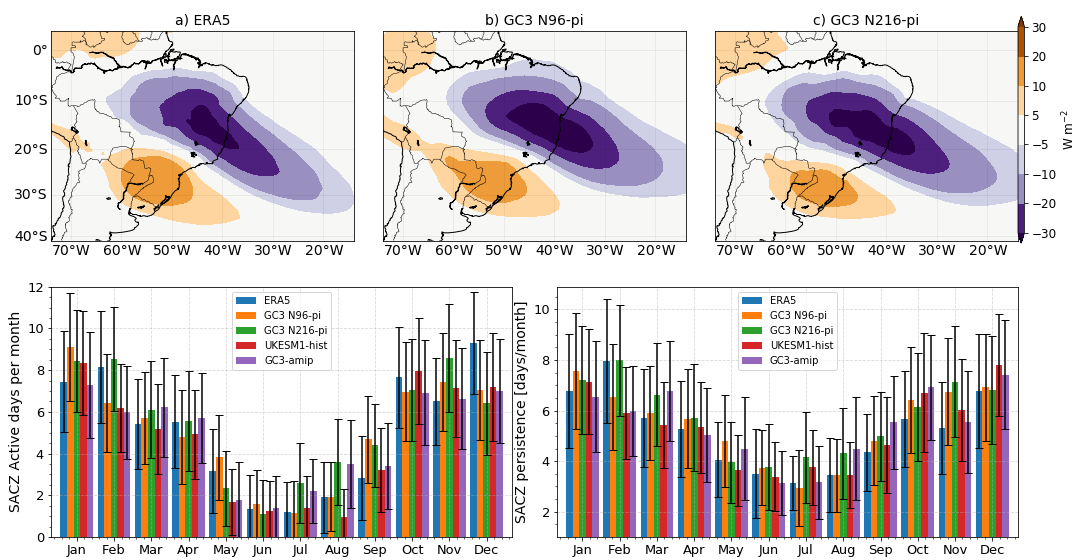
\includegraphics[width=\linewidth]{figures/saczanalysis.png}
\caption{(a, b, c) OLR anomalies during active South Atlantic Convergence Zone (SACZ) events. (d, e) Frequency of active SACZ days and length of active SACZ events in reanalysis and model data, the standard deviation is shown as the error bar. The SACZ active days are constructed by first computing the first EOF of the monthly-mean deseasonalized OLR and then the daily OLR, previously filtered to remove periods higher than 99 days, is projected on the EOF pattern to produce a time-series of pseudo-principal components. Active SACZ days are found when this time-series of pseudo-PCs is greater than 1, and the persistence is measured as the number of continuous days where the time-series is greater than 1.}
\label{fig:sacz}
\end{figure}

 The South Atlantic Convergence Zone (SACZ) is a nortwest-southeast oriented band of convection and is a prominent influence on the South American Monsoon mean and extreme rainfall \citep{carvalho2004,marengo2012,jorgetti2014}. The SACZ is primarily characterized by convergence oriented northwest-to-southeast that promotes rainfall in southeastern Brazil. The position of the SACZ and strength are an important factor for variability of the South American monsoon on different temporal and spatial scales \citep{carvalho2004,marengo2012,jorgetti2014}. 
 
 The SACZ in this simulations, defined by the out-going longwave radiation empirical orthogonal function analysis (Figure \ref{fig:sacz}) closely resembles the pattern found in ERA5. The SACZ active days and the persistence of the SACZ are also compared and found to be in relatively good agreement between reanalysis and model datasets.
The simulations from UKESM1, and GC3 N96 and N216 appear to reasonably simulate the spatial pattern of active SACZ days characterized by the low OLR in southeastern Brazil and higher OLR in the La Plata Basin. Similarly, the seasonal cycle of the frequency and persistence of SACZ active days is very well represented by the models with peak activity found from November through January and very little activity during austral winter. The impact that an accurate representation of the SACZ activity in GCMs has for representing short-scale variability of the South American Monsoon System is an open question, as the SACZ is rarely assessed in CMIP analyses.




\section{Precipitation and convection in the AMS}\label{sq:precip}
%This section compares the spatial and temporal distribution of rainfall in four key regions of the AMS between observations and reanalysis, and the simulations, as well as other characteristics of convective activity, such as height and strength. %, are compared to better understand convective representation in this region.

\subsection{Mean seasonal precipitation}

\begin{figure}[t!]
\centering
 %\noindent
 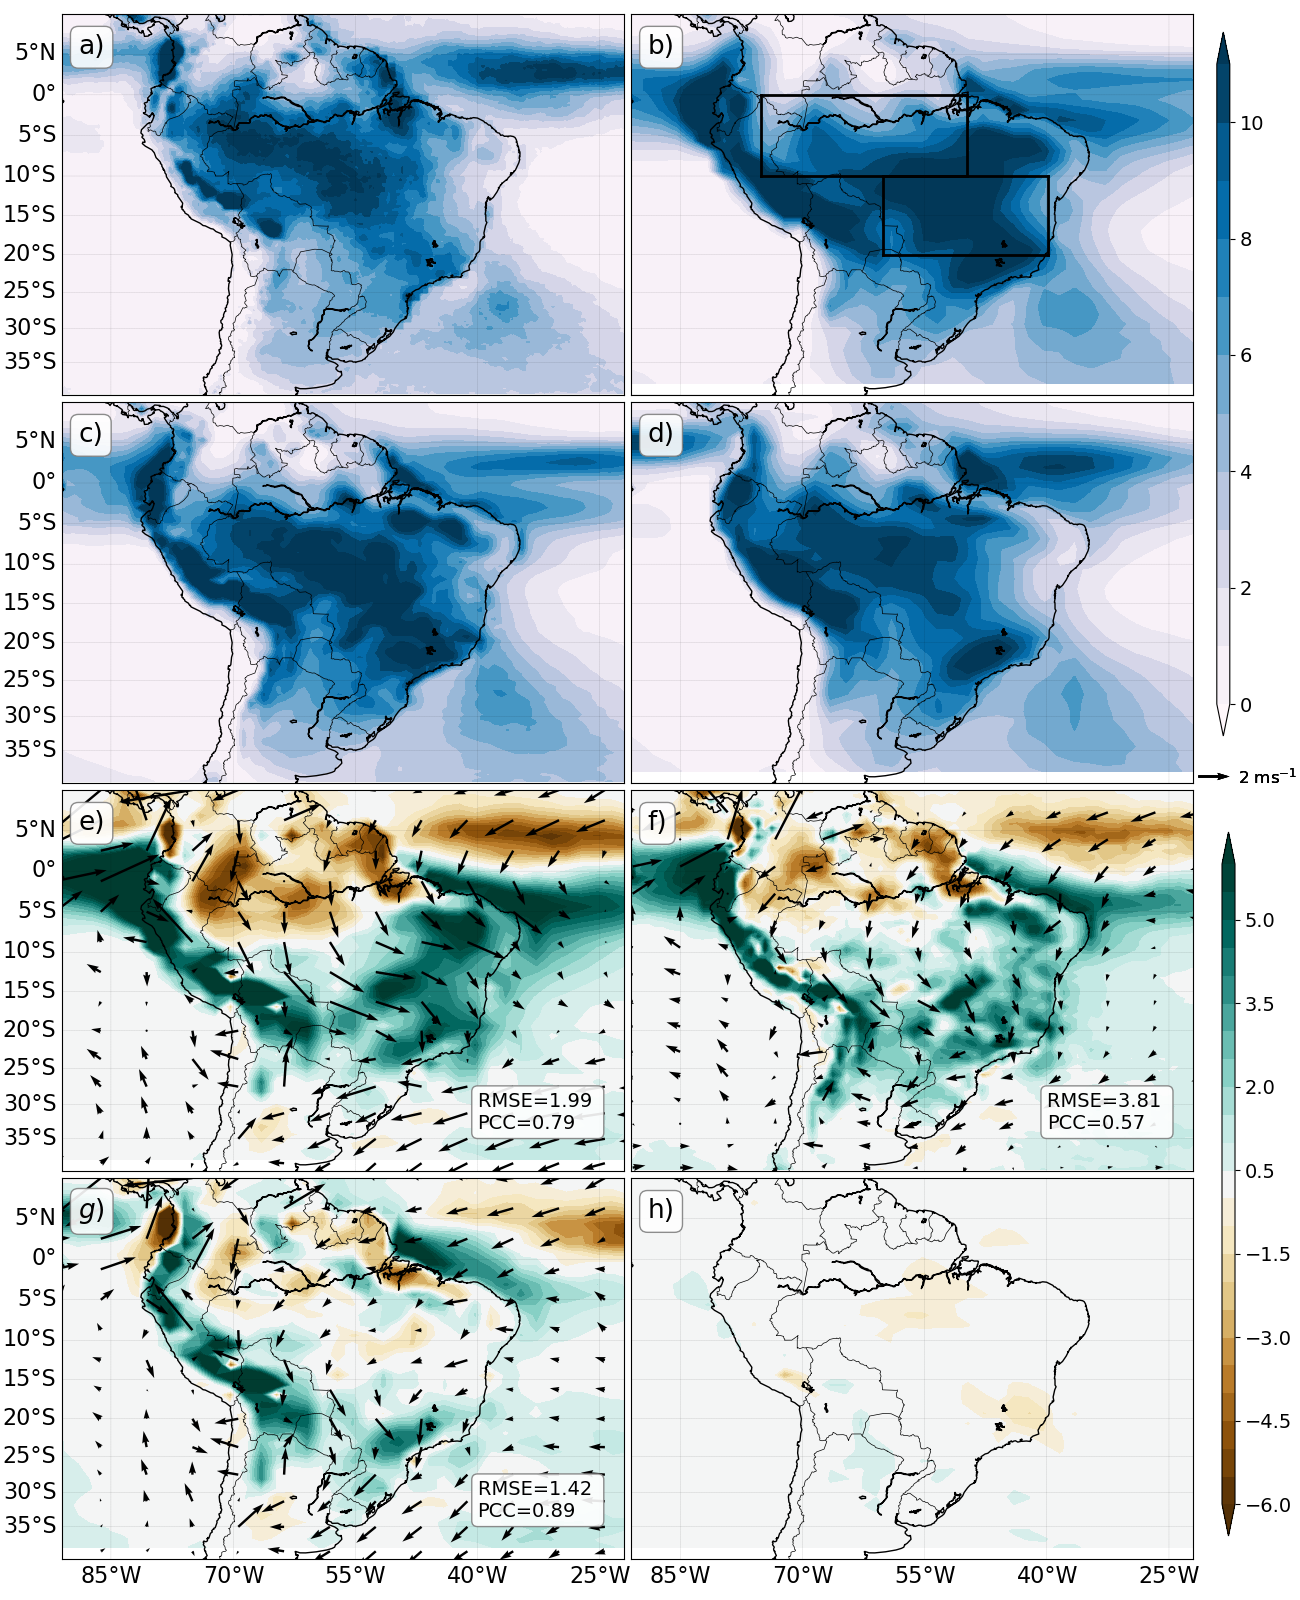
\includegraphics[width=0.875\linewidth]{figures/fig6.png}
\caption{ DJF mean rainfall [mm day$^{-1}$] from (a) TRMM, (b) UKESM1-historical, (c) GC3 N216-pi and (d) GC3-amip. (e, f, g) show the statistically significant differences between panels (b, c ,d) and (a) TRMM, respectively. (h) Precipitation difference between UKESM-historical and  UKESM1-pi, only statistically significant differences (95\%) confidence level is shown.  The biases in the 850-hPa winds are shown as vectors. }
\label{fig:6}
\end{figure}

  The austral summer (DJF) rainfall distribution in South America of the TRMM dataset and the simulations for GC3 N216-pi, UKESM-hist and GC3-amip (Figure \ref{fig:6}) shows several noteworthy biases in the coupled simulations. 
The maximum austral summer rainfall in TRMM
(Figure \ref{fig:6}a) is found as a northwest-southeast oriented band of precipitation from the core Amazon region into southeastern Brazil, which is related to the SACZ.
The biases are illustrated (Figures \ref{fig:6}e-h) as the precipitation difference between the simulations and TRMM.
 
%The coupled simulations (e.g. Figure \ref{fig:6}b, c) overestimate rainfall in southeastern Brazil and underestimate rainfall in the core Amazon region.
 

   The coupled simulations show three main biases.
Rainfall in the Atlantic ITCZ in these simulations is displaced southwards, observed as positive (+5 mm day$^{-1}$) biases south of the equator and negative biases ($-$5 mm day$^{-1}$) north of the equator in the Atlantic.
Second, the models underestimate rainfall in the core Amazon basin by $-$3 mm day$^{-1}$ on average, and the third major bias is that rainfall in southeastern Brazil is overestimated by more than +5 mm day$^{-1}$, approximately +100\% of the observed rainfall in this region.  

 The precipitation biases are associated with a stronger northerly flow in South America, transporting moisture from the Amazon into southeastern Brazil and the La Plata Basin.   
The magnitude of these biases is smaller in GC3 N216 (Figure \ref{fig:6}f) than in the low resolution simulations, such as UKESM1-hist.   The ensemble mean GC3 AMIP (Figure \ref{fig:6}d) shows a better representation of the austral summer rainfall and circulation patterns, removing the main circulation biases (Figure \ref{fig:6}g) of the coupled simulations.   
The response to historical forcing, illustrated by the difference between UKESM1-hist and UKESM1-pi (Figure \ref{fig:6}h), is much weaker than the magnitude of the biases and is characterized by a weak drying of the Amazon and southeastern Brazil.


\begin{figure}
\centering
 %\noindent
 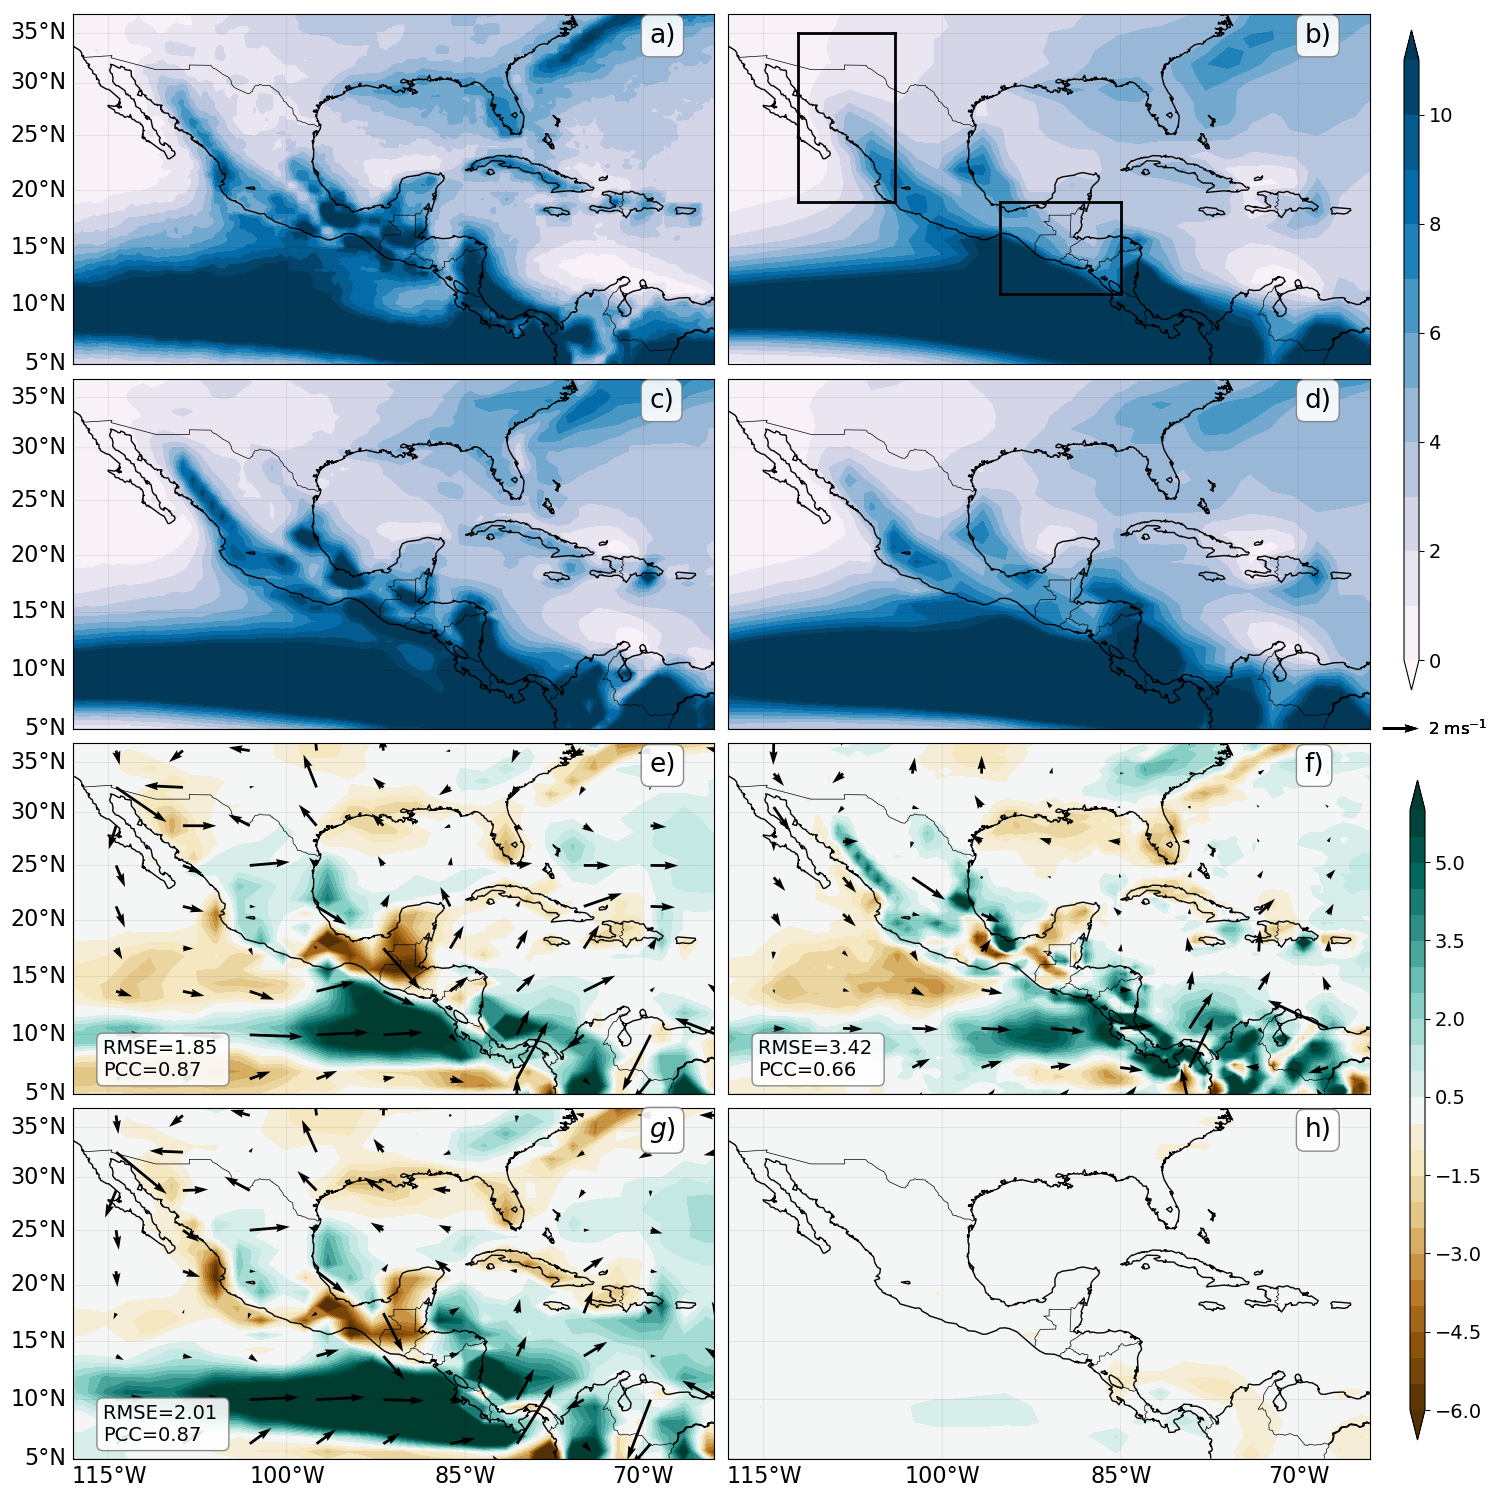
\includegraphics[width=\linewidth]{figures/Fig8.png}
\caption{ As in Figure \ref{fig:6} but for JJA in the northern part of subtropical America.   }
\label{fig:7}
\end{figure}

The modelled and observed JJA mean rainfall and biases for Mexico and Central America are shown in Figure \ref{fig:7}.
The main feature is the East Pacific (EP) ITCZ which extends north to 15$^\circ$N near the western coast of Mexico as a broad band of rainfall (>11 mm day$^{-1}$).
 The modelled EP ITCZ (Figures \ref{fig:7}e, f, g) rainfall is overestimated by more than 5 mm day$^{-1}$, especially in GC3-amip. This wet bias is associated with a westerly bias in the low-level circulation, suggesting a weaker flow from the Caribbean into the East Pacific.

The North American Monsoon can be observed as a band of precipitation across western Mexico. In the core monsoon region, near the Sierra Madre Occidental \citep{adams1997, zhou2016}, the JJA-mean rainfall is higher than 8 mm day$^{-1}$. %Several regions in southern Mexico also exhibit large seasonal mean rainfalls.
The distribution of rainfall in the North American Monsoon region is relatively well represented in all the simulations, as only a moderate wet bias (+2 mm day$^{-1}$) in western Mexico is observed.
The northernmost part of the North American Monsoon (southwestern US) is best simulated by GC3 N216-pi, as the other simulations show a dry bias in this region.
%This positive bias extends to southern Central America.
The low-resolution simulations (Figure \ref{fig:7}e) underestimate rainfall (-5 mm day$^{-1}$) over land in southern Mexico, Guatemala and Belize.
Rainfall in the Caribbean islands and Florida is underestimated (-1 mm day$^{-1}$) in all simulations.

In most cases for JJA in this region, the precipitation and wind biases were reduced in the high-resolution simulation (Figure \ref{fig:7}f) and little-to-no difference was observed between UKESM1-hist and GC3-hist (not shown).
The precipitation response to historical forcing is much lower than the biases (Figure \ref{fig:7}h) with no significant precipitation differences over land due to the historical forcing. % shows a decrease in precipitation.
 

\subsection{The annual cycle of rainfall}\label{sq:raincycle}

\begin{figure}[b!]
\centering
 %\noindent
 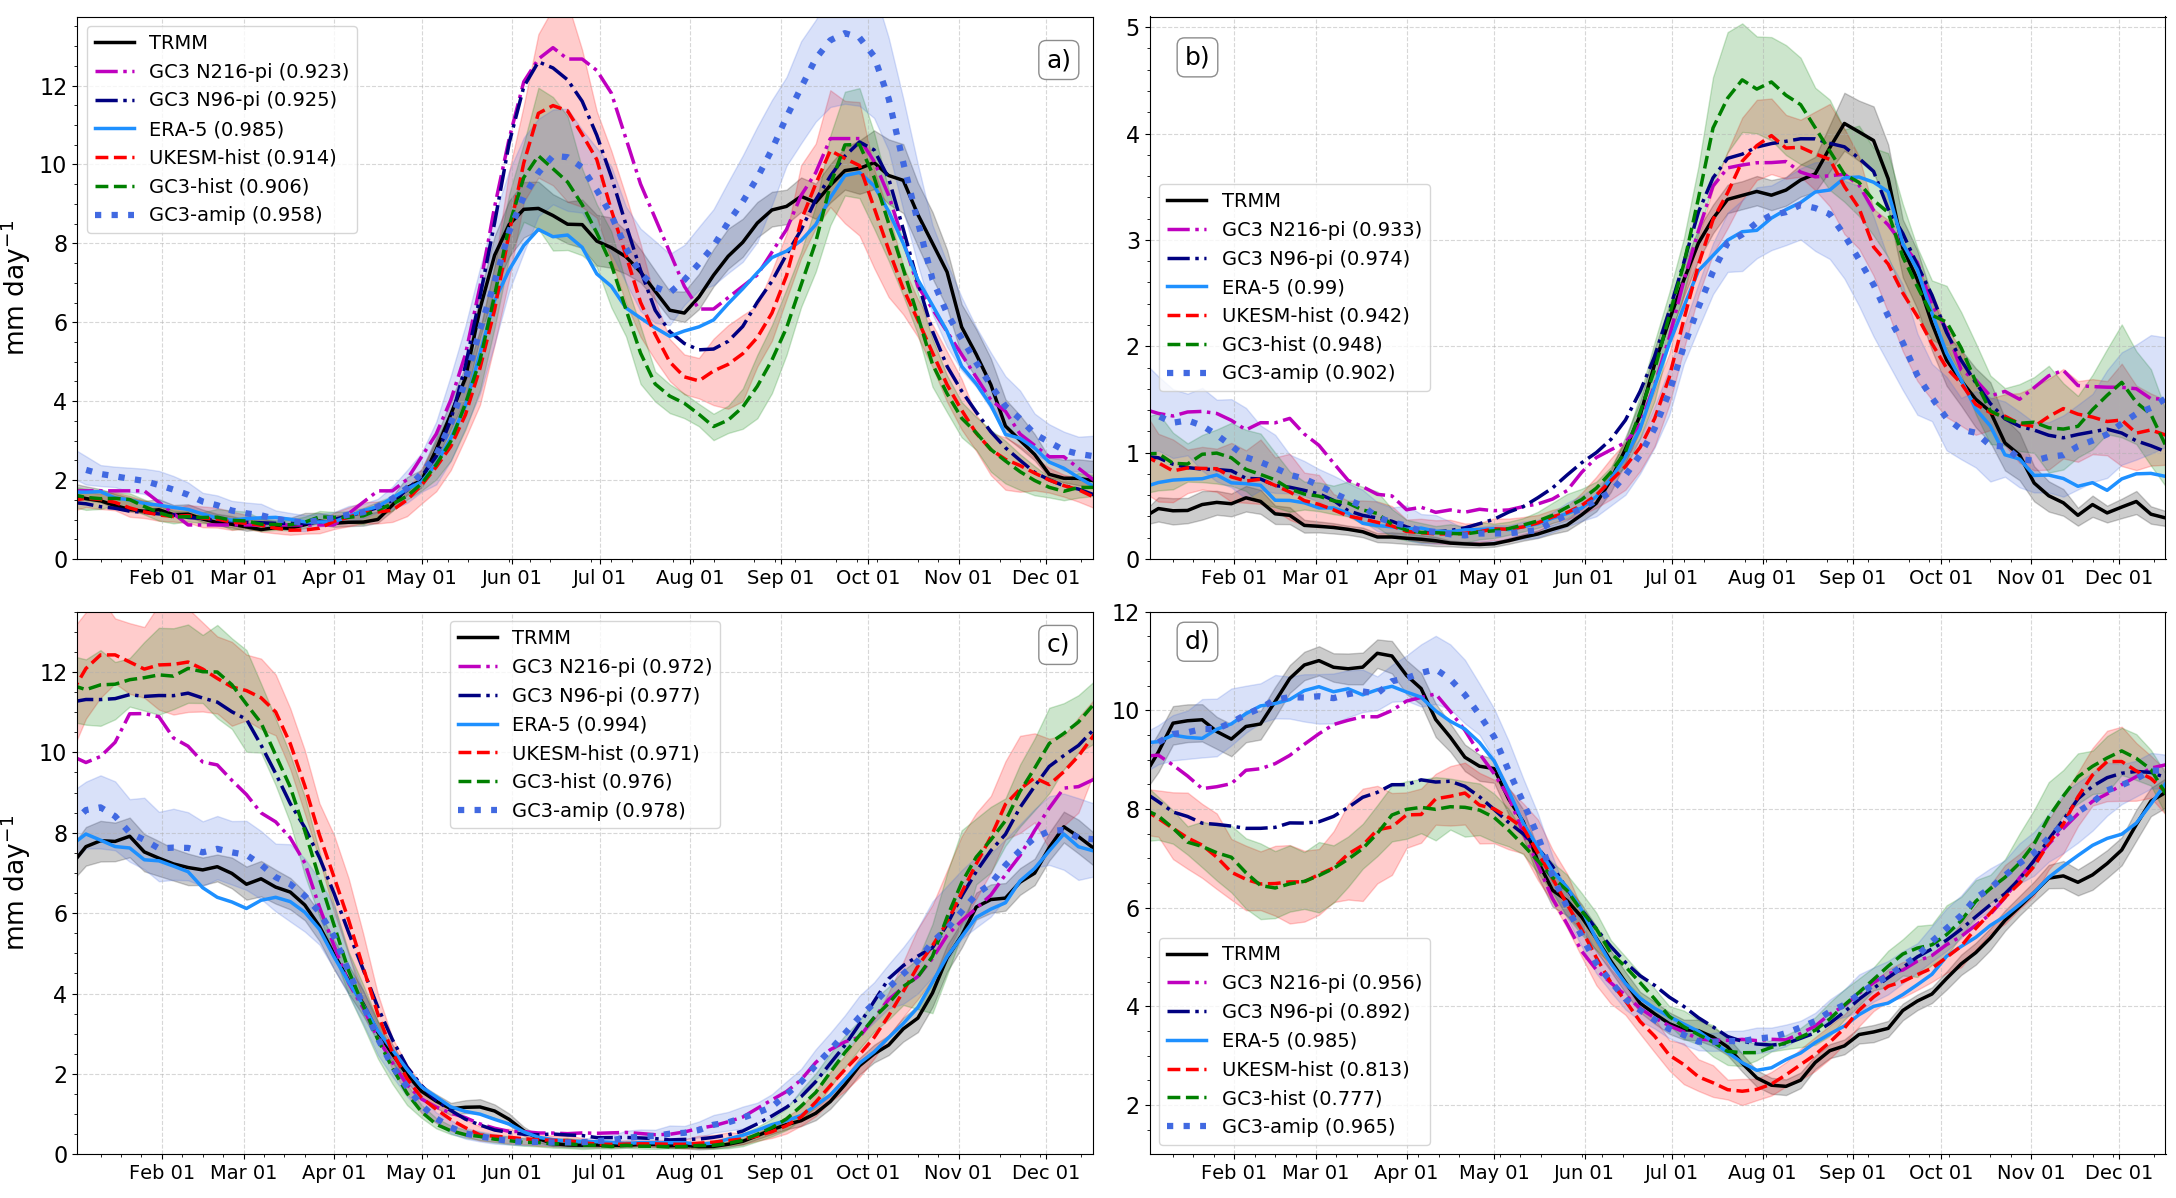
\includegraphics[width=1.0\linewidth]{figures/amipseasonalcycle.png}
\caption{Annual cycle of pentad-mean rainfall in the regions (a) the Midsummer drought, (b) the North American Monsoon, (c) Eastern Brazil and (d) the Amazon Basin. The regions are defined as in Figure \ref{fig:2} and are illustrated in Figure \ref{fig:7}b and Figure \ref{fig:8}b. The shaded regions represent observational uncertainty for TRMM and ensemble spread for the historical experiments. The correlation coefficient for each of the simulated seasonal cycles with TRMM is given in brackets in each panel.  }
\label{fig:8}
\end{figure}

%CMIP assessments typically evaluate rainfall model performance by inspecting area-averaged monthly-mean evolution of rainfall.
%However, this temporal resolution is not enough to properly evaluate the performance of a simulation, particularly in monsoonal regions where the dates of monsoon onset and demise have relevance for sectors such as agriculture.

Figure \ref{fig:8} shows the seasonal cycle of rainfall at the pentad (5-day) scale over the North American Monsoon, the  Midsummer drought (MSD), the Amazon and eastern Brazil regions. The correlation between TRMM and the model and reanalysis data (ERA5) is also shown in each panel. 


The seasonal cycle of precipitation in the MSD region in the simulations is well represented as all the simulations show the characteristic bimodal distribution, a feature that is uncommon for a climate model to be able to reproduce \citep{ryu2014}.
%This peculiar bimodal distribution of rainfall is characterised by a first rainfall maxima in June and a second maximum in late September, separated by a relatively drier period with a minimum at the start of August. The Midsummer drought bimodal distribution was only found in a handful of CMIP5 models \citep{yin2013}.
However, the characteristics of the simulated MSD are different from observations.
For example, the magnitude of the first peak and second peaks in the simulations are different. 
For instance, most of the first peak simulated magnitudes are higher than TRMM by 4 mm day$^{-1}$, and the AMIP simulation overestimates the second maximum of rainfall by 2-3 mm day$^{-1}$. Similarly, the differences between the first peak and the MSD and between the MSD and the second peak are more pronounced in the coupled simulations. The timing of the MSD period is different in the models, as the simulations show the driest period taking place 10 days after TRMM and ERA5. %  All the simulations show different magnitudes of the first and second peak and the MSD precipitation, 
 
 

In the North American Monsoon (Figure \ref{fig:8}b), the observed seasonal cycle is characterized by a very long and dry period ranging from the end of November to the start of June, which is followed by a sharp increase of rainfall around mid-June. The timing of the increase of rainfall in models coincides with observations, suggesting that onset timing and strength is well represented in these models.
Moreover, the modelled and observed mean precipitation rates during monsoon maturity are $~$4 mm day$^{-1}$, from mid-July until early September, which suggests notable ability of the models to reproduce the peak monsoon rainfall.
%The timing of monsoon retreat is also well represented by the simulations, as both modelled and observed rainfall decay during September.
   The historical simulations show a shorter wet season characterised by an earlier retreat of the monsoon rainfall and, as all the simulations, a positive boreal fall rainfall bias (+1 mm day$^{-1}$), a feature that has been shown in these models in CMIP5 \citep{geil2013}. % and that will be further explored in the following chapter. %For instance, GC3-hist retreats on average around August 16th. 
%However, winter-time rainfall, before monsoon onset and after monsoon retreat, is overestimated by all the simulations, particularly the higher resolution GC3.1 N216 which has a positive bias of $~$2 mm day$^{-1}$ in early winter. 


The seasonal cycle of precipitation in eastern Brazil is characterised by a very wet summer ($\sim$8 mm day$^{-1}$) compared to a very dry ($\sim$0.2 mm day$^{-1}$) winter (Figure \ref{fig:8}c).
%The South Atlantic Convergence Zone has a centre of action over this region and thus controls several aspects of precipitation \citep{carvalho2004,marengo2012}.
Rainfall in TRMM and ERA5 increases steadily from austral spring (September) to a maximum found in early January ($\sim$8 mm day$^{-1}$).
Rainfall in this region decreases to $\sim$6 mm day$^{-1}$ by late March as the monsoon migrates northward and then sharply decreases in austral fall.


The models (Figure \ref{fig:8}c) show a positive bias during monsoon maturity. This bias was found to be of +4 mm day$^{-1}$ and +2.5 mm day$^{-1}$ for the low and medium resolution simulations, respectively.
This positive bias in the maximum rainfall is consistent with the biases shown in Figure \ref{fig:6}, which showed that rainfall in southeastern Brazil is overestimated, especially in the low resolution coupled simulations.   In contrast to the coupled simulations, GC3-amip shows a very good agreement with the observed maximum summer rainfall and the seasonal cycle (r=0.978) throughout the year.
%In spite of this positive bias in the magnitude of precipitation, the seasonal evolution of rainfall is very well represented by the simulations, as the onset and retreat dates are in close agreement with the observations.

Finally, the seasonal cycle in the Amazon (Figure \ref{fig:8}d) has a weaker contrast as rainfall greater than 2 mm day$^{-1}$ is found year-round. The coupled simulations show a dry bias during austral summer and a good agreement with the observations during austral winter. Rainfall rates in the Amazon from January to March, in both TRMM and ERA-5, is close to 10 mm day$^{-1}$, yet the low resolution simulations show rainfall rates of 8 mm day$^{-1}$ in mid-February, particularly the historical experiments.
GC3 N216-pi shows a better agreement with observations but still underestimates summertime rainfall by 1 mm day$^{-1}$.   

This dry Amazon bias has been a known feature of GCMs, including the MOHC models, since CMIP3 \citep{li2006,yin2013}. In these simulations the dry Amazon bias is only alleviated in GC3-amip whose seasonal cycle and maximum summer rainfall agree well with observations.   
% Peak summertime rainfall is underestimated by the coupled model simulations, particularly the historical experiments. 
The models, however, represent with reasonable skill the timing of the transition from
early austral spring (4 mm day$^{-1}$ in September) to summertime rainfall (6 mm day$^{-1}$ in November).
%The low resolution simulations, after simulating an annual maximum of rainfall in December, simulate a decrease in precipitation for January and February, whereas the observations show the opposite behaviour.


\subsection{Characteristics of convective activity}




The seasonal cycles of out-going longwave radiation (OLR), vertical velocity ($\omega$) and specific humidity ($q$) are key features of a monsoon since these quantities characterise the strength and height of deep convection, as well as the moisture within the column.
 shows The pentad-mean annual cycle of OLR, $q$ and $\omega$ at the 500-hPa level in four regions of the AMS (Figure \ref{fig:9}) are used as process oriented diagnostics to further evaluate the biases in the spatial distribution and seasonal cycle of rainfall.
 

For the North American Monsoon the seasonal cycle of OLR, $q$ and $\omega$ is relatively well represented in the simulations.
During late boreal winter and early spring, OLR increases steadily as a result of surface warming.
However, in early June, near the onset date \citep{douglas1993,geil2013}, OLR sharply decreases reaching a minimum value of 246 W m$^{-2}$ by mid-July.
The vertical velocity decreases steadily from January to a minimum in August, indicating ascent from May 1st until September 15th.
 The models show similar seasonal cycles but overestimate the summertime OLR by $\approx$ 6 W m$^{-2}$ and underestimate mid-level moisture by 0.3 g/kg and $\omega$ by 0.01 Pa s$^{-1}$. 
%After convective activity decreases in late August in ERA-5, OLR increases to a local maxima of $\sim$ 271 W m$^{-2}$ on mid-September, $q$ decreases significantly and $\omega$ turns positive.
The simulated shallower convection and drier mid-troposphere is seemingly compensated by stronger mid-level ascent.
%During boreal fall, OLR decreases again due to the temperature seasonal cycle in the region and moisture remains low.

\begin{figure}[t!]
\centering
 %\noindent
 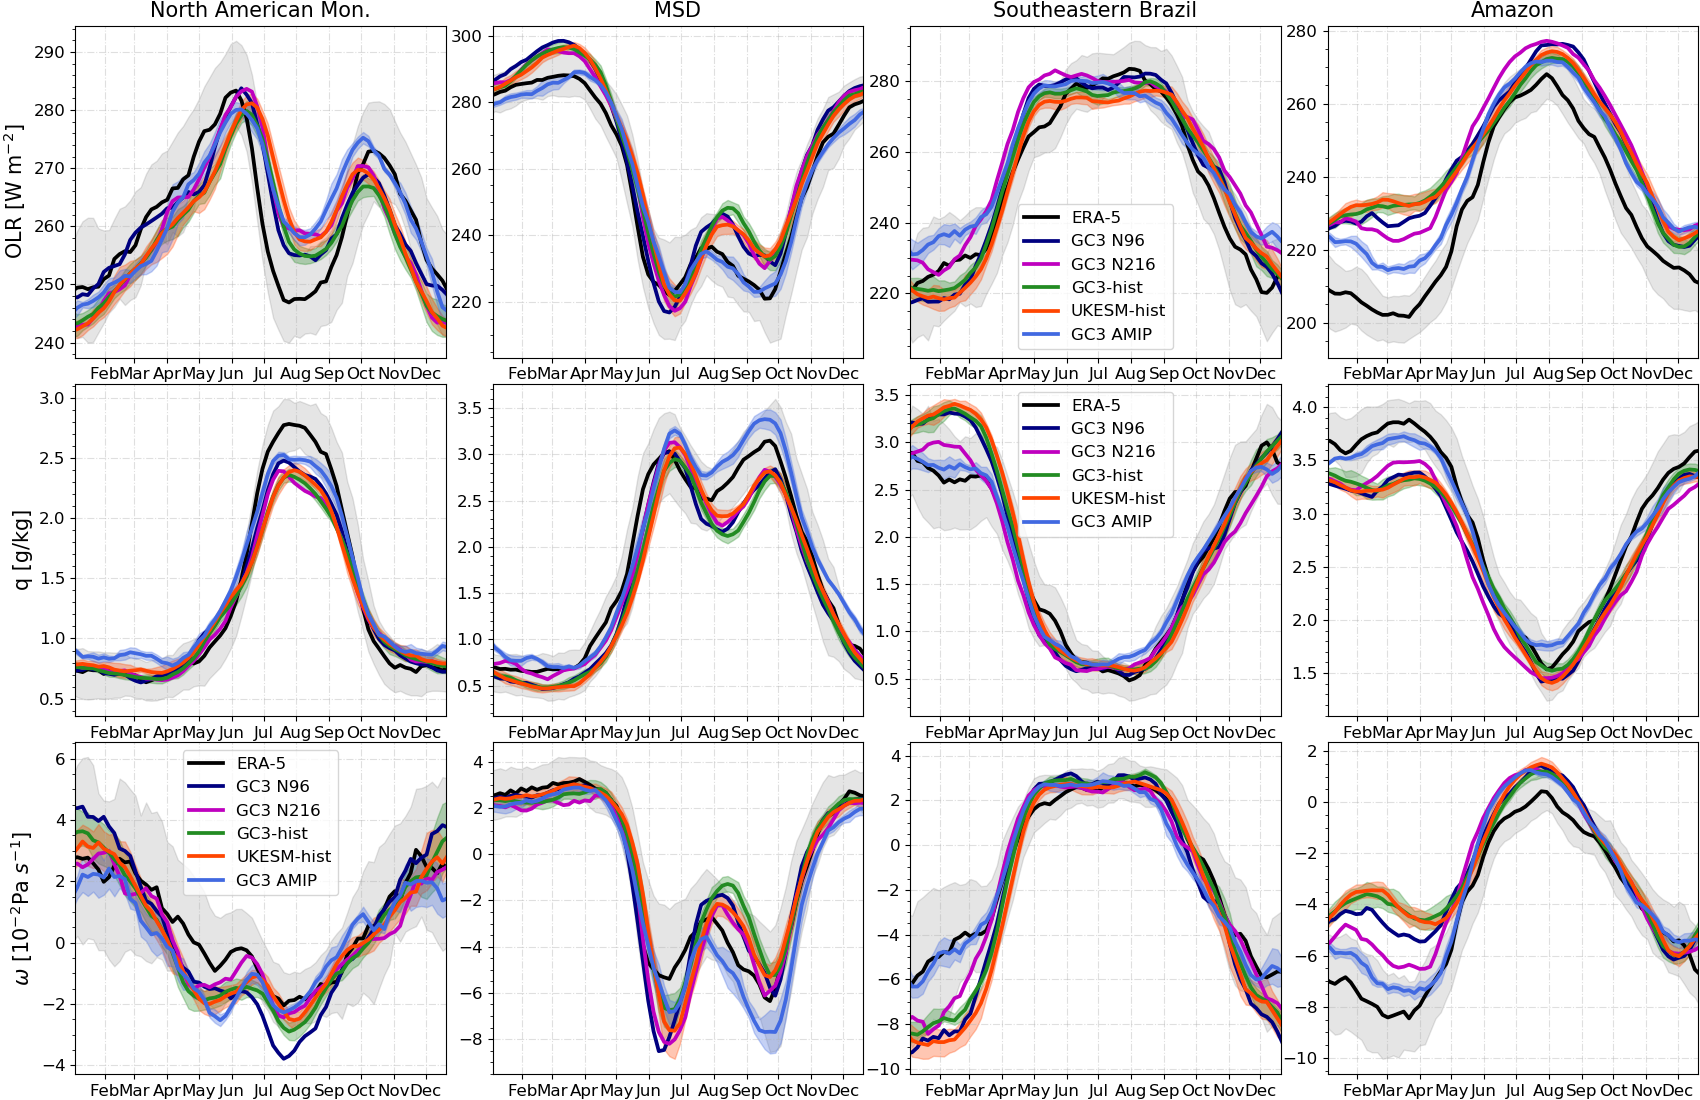
\includegraphics[width=\linewidth]{figures/fig9b.png}
\caption{Pentad-mean (upper) out-going longwave radiation (OLR), (middle) specific humidity at 500-hPa and (lower) $\omega$ 500-hPa. These are shown from left to right for the North American Monsoon, the Midsummer drought, southeastern Brazil and the core Amazon. The uncertainty in ERA-5 data, shown as faint gray shading was estimating by bootstrapping with replacement the ERA-5 record 10,000 times. }
\label{fig:9}
\end{figure}

In the MSD region, OLR and $q$ show signs of convective activity from mid-April, as OLR sharply decreases and moisture increases.
%The key characteristic of the MSD is the modest decrease in rainfall in the midsummer.
The characteristic MSD bimodal distribution of precipitation can also be observed as two peaks of low OLR, high $q$ and low $\omega$.
These periods are separated by a period of relatively higher OLR, lower $q$ and weaker ascent from June 15 until late August.
%The reanalysis data shows that during the MSD period OLR increases by 10 W m$^{-2}$, $\omega$ decreases by 0.015 Pa s$^{-1}$ and $q$ decreases by 0.5 g/kg.
Although arguably with a small dry bias with shallower convection after mid-July, the simulations follow closely the observed seasonal cycle.

The simulated conditions during the first peak period show similar OLR and mid-level moisture but stronger ascending motions, which may explain the positive rainfall bias in this period showed in Figure \ref{fig:8}a.
In the period between the first peak and the MSD, the simulated OLR increases more sharply than observations from 220 W m$^{-2}$ (June 15) to 250 W m$^{-2}$ (early August), with similar behaviour in $\omega$ and $q$, which may also be related to the strong MSD precipitation differences described in the previous section.
%In the same period, the simulated moisture and ascent decrease more sharply than observations, in agreement with the stronger variations of precipitation (Figure \ref{fig:8}a).
%The stronger than observed changes to the characteristics of convection are consistent with the sharper than observed midsummer drought in the simulations showed in Figure \ref{fig:8}a.
The period during the second peak of rainfall in September shows signs of shallower convection and a drier mid-level when compared to ERA5.
%The characteristics of the retreat stage of rainfall at the start of October shows close agreement between reanalysis and simulations.
%Overall, the models seem to reproduce the annual cycle of OLR and

In southeastern Brazil, the simulations reasonably follow the timings of the annual cycle of OLR, $q$ and $\omega$ of the reanalysis, particularly during austral winter. The moisture $q$ in ERA5 during  the dry seasons of austral fall, winter and spring is reasonably simulated by all the experiments. However, during austral summer, the coupled model simulations show significant biases characterised by stronger ascent and increased specific humidity in the mid-levels, although the height of convection (OLR~ 225 W m$^{-2}$) is only modestly higher in the simulations.

%The seasonal cycle of these proxies for convective activity in the Amazon basin are shown by Figure \ref{fig:8}.
The simulated OLR, q and $\omega$ exhibit the highest biases in the Amazon. During austral summer, particularly January and February, the simulated convective activity is shallower (OLR bias of +25 W m$^{-2}$) and weaker (positive $\omega$ bias +0.02 Pa s$^{-1}$) and the mid-level troposphere is drier (~-0.5 g/kg) than in ERA5. All these biases are in agreement with the dry Amazon bias described in the previous section. In spite of biases in the magnitude of OLR, $q$ and $\omega$ during peak convective activity, the seasonal variation is very well simulated so that convective activity, as evidenced by these metrics, starts and ends in the simulations within one or two pentads of the reanalysis. The smallest biases in coupled simulations are those of GC3 N216-pi, not just for the Amazon region but for the other regions as well.  The simulated OLR, $q$ and $\omega$ in GC3-amip in southeastern Brazil and the Amazon show a much better agreement with the reanalysis during austral summer than the rest of the simulations.


\section{ENSO Teleconnections}\label{sq:enso1}





El Ni\~no-Southern Oscillation (ENSO) teleconnections are the prominent source of interannual variability for the AMS \citep{vera2006}, as summarized in section \ref{sub:lit_enso}.
The response to ENSO events in UKESM1 and HadGEM3 is investigated in this section, which first shows the temperature, sea-level pressure (SLP) and precipitation responses  to observed and simulated ENSO events in the AMS, to then analyse the effect of ENSO flavours on the AMS. Finally, results show a possible influence of the QBO for the teleconnections of ENSO. 

%Throughout this section, ENSO events were defined when the DJF-mean Ni\~no 3.4 index was above or below 0.65 \citep{trenberth1997}.   



\subsection{Canonical teleconnections}

\begin{figure}[t!]
\centering
 %\noindent
 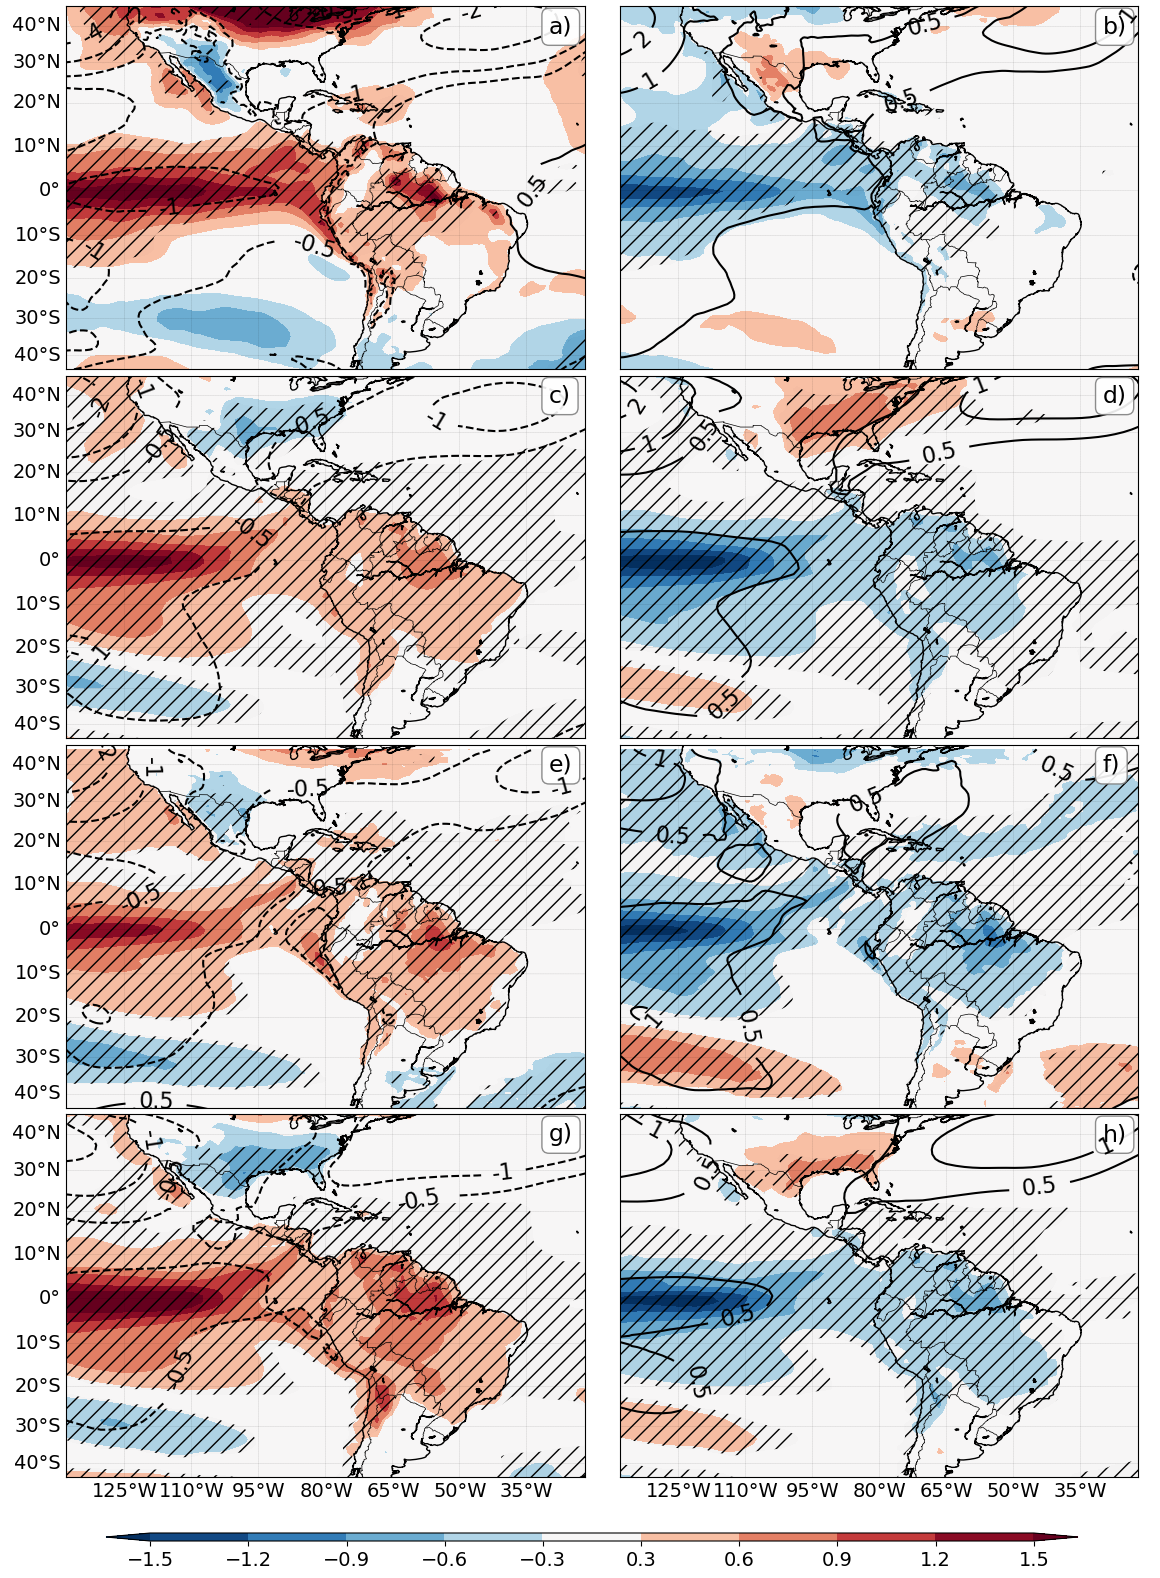
\includegraphics[width=0.89\linewidth]{figures/ensotemp_3}
\caption{ DJF Temperature anomalies (colour contours in K) and SLP (line contours in hPa) during (a, c, e, g) El Ni\~no and (b, d, f, h) La Ni\~na events. Results are shown for (a, b) ERA-5, (c, d) UKESM1-hist, (e, f) GC3 N96-pi and (g, h) GC3 N216-pi. The hatched regions denote differences between ENSO phases and the climatological state with significance to the 99\% confidence level from a Welch t-test for the temperature field. }
\label{fig:10}
\end{figure}

The surface temperature and sea-level pressure (SLP) responses to ENSO events are shown in Figure \ref{fig:10} for HadGEM3, UKESM1 and ERA5 data during DJF, the season of strongest impact of ENSO events.
The characteristic warm anomaly during El Ni\~no events in the East Pacific Ocean does not extend to the east in all the simulations as the observed warm anomaly. In turn, the cold anomalies during La Ni\~na events in the Central Pacific are colder in the simulations than in ERA5. 
The teleconnection to southern North America, i.e., colder (warmer) conditions in southern (northern) North America during El Ni\~no events is relatively well simulated. For example, the simulated and observed teleconnection patterns to South America, e.g., the cold anomalies during La Ni\~na events in northern South America are well simulated. However, the low resolution simulations show a broader and stronger than observed negative response in southeastern US to El Ni\~no events. 

%The simulated teleconnection pattern to North America is better represented in GC3 N216-pi. % It is worth noting that the medium resolution simulations seems to simulate stronger El 

\begin{figure}[t!]
\centering
 %\noindent
 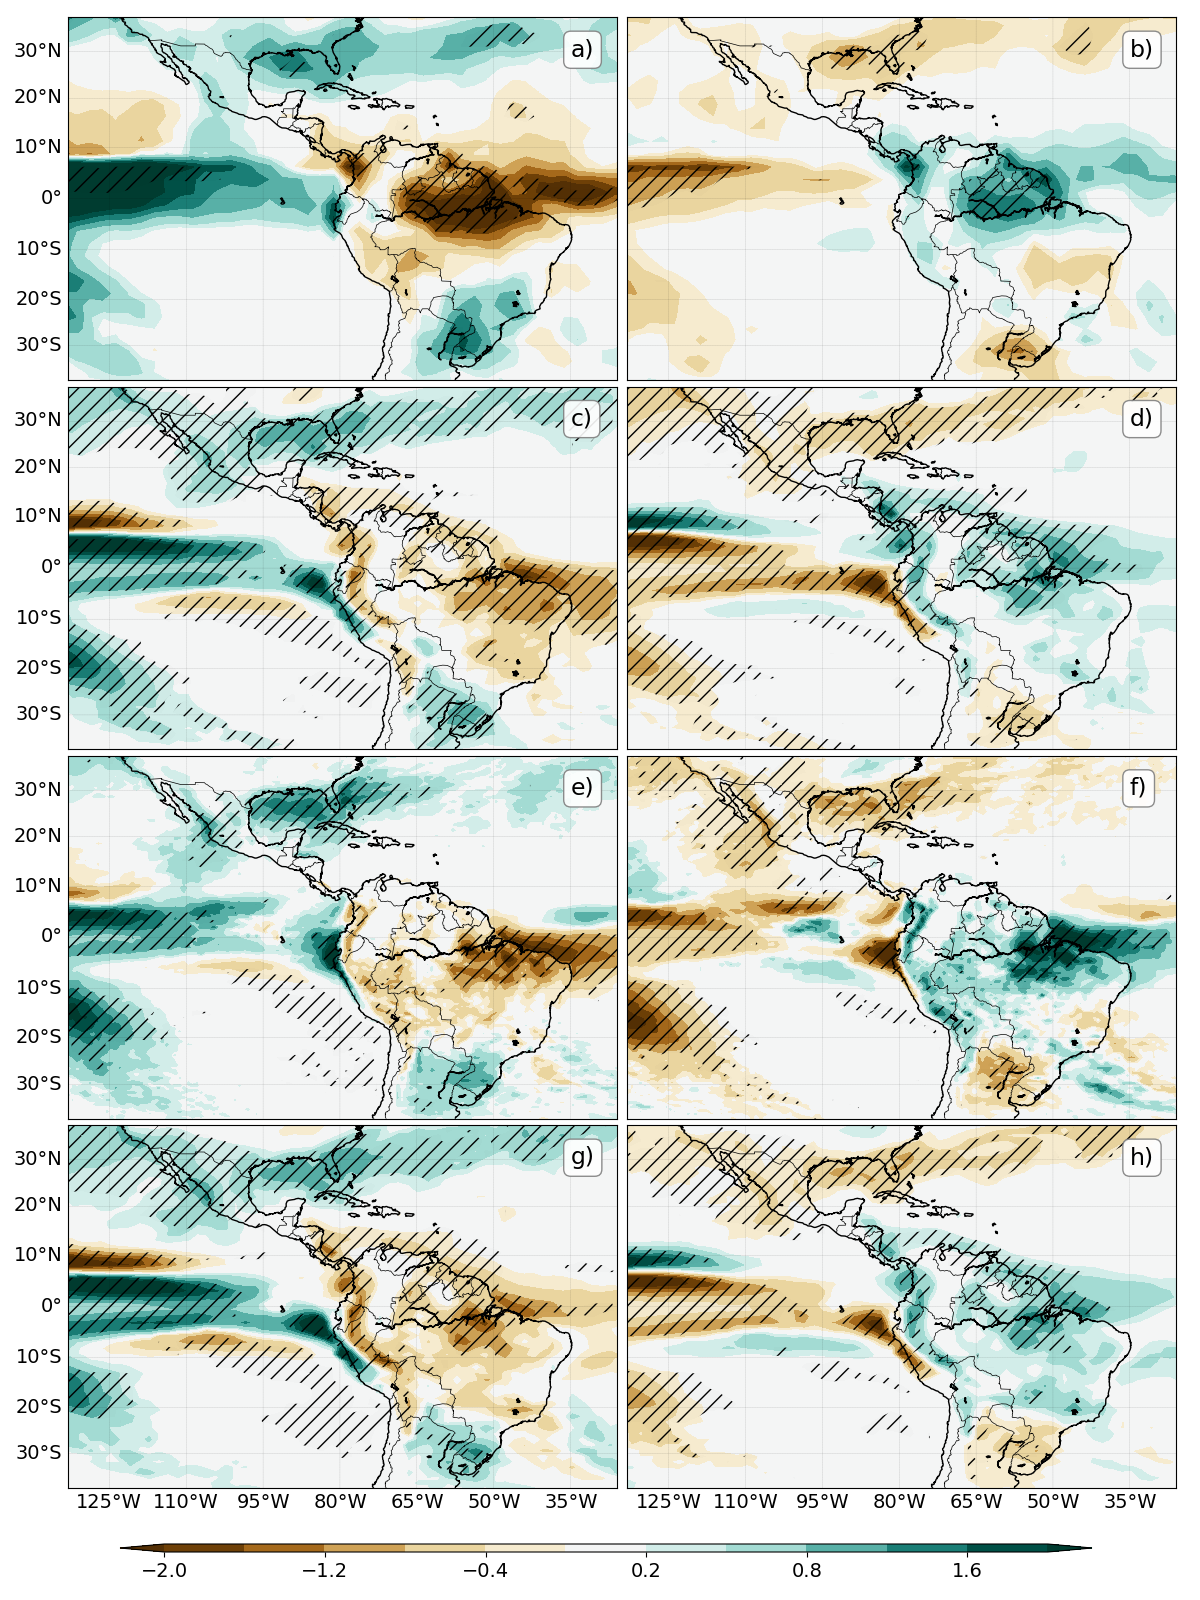
\includegraphics[width=0.881\linewidth]{figures/ensopr_3}
 \caption{As in Figure \ref{fig:10} but for the rainfall response [mm day$^{-1}$] using GPCP as the observational dataset.}
%\caption{ Precipitation  DJF response to (a, c, e, g) El Ni\~no and (b, d, f, h) La Ni\~na events in (a, b) GPCP, (c, d) UKESM1, (e, f) GC3.1 N96 and (g, h) GC3.1 N216. The hatched regions denote 99\% significance from a Welch t-test. }
\label{fig:11}
\end{figure}

The SLP response in the north Pacific and North America, known as the Pacific North-American pattern, is linked with a displacement of the subtropical jet affecting the eastward propagation of wave activity that reaches the North Atlantic  \citep[e.g.][]{bayr2019,jimenezesteve2020}.
During  El Ni\~no events, the Aleutian Low is strengthened in ERA5, with a strong SLP anomaly (-4 hPa) off the coast of California. The models show a similar but smaller SLP response in the same region.  El Ni\~no events events are associated with a negative phase of the North Atlantic Oscillation (NAO), with an opposite response for La Ni\~na events. While the models seem to be able to capture this response of the NAO, the simulated response is weaker than observed.   A sensible representation of the ENSO-NAO tropospheric teleconnection may be relevant to then simulate the effect of the NAO on Central American and northern South American rainfall \citep{giannini2000,giannini2004}.  




\begin{figure}
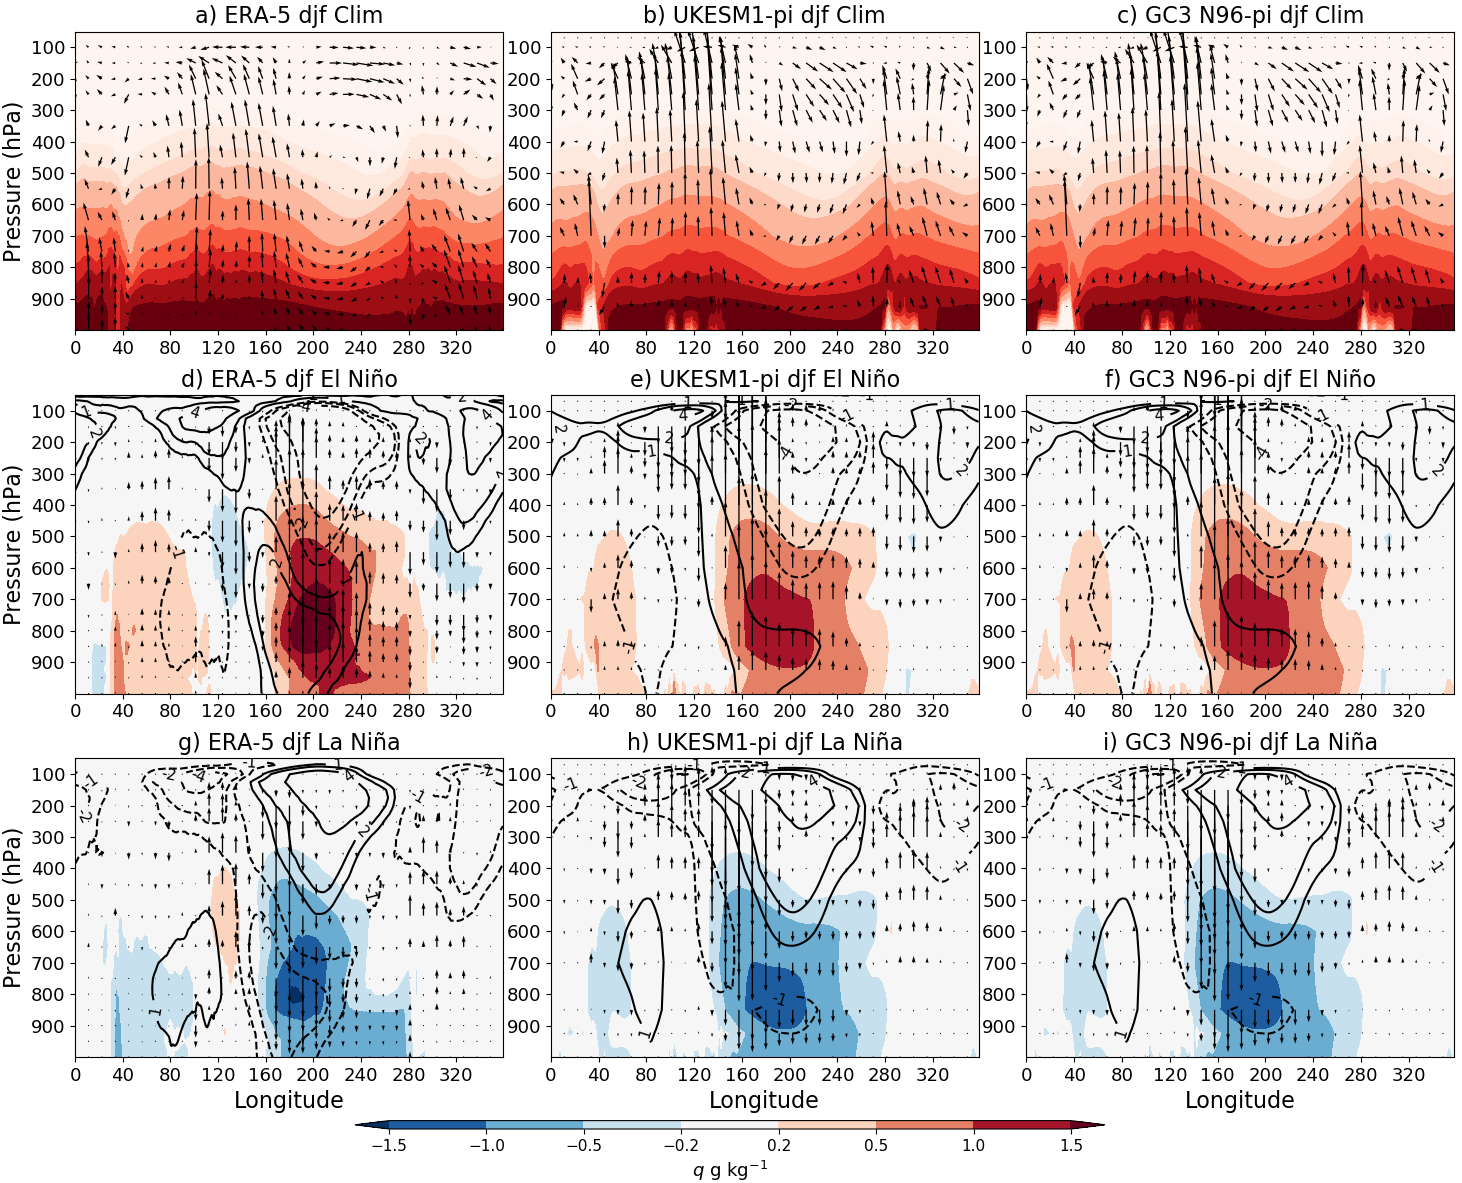
\includegraphics[width=\linewidth]{figures/walkerfinal}
\caption{DJF Longitude-height Walker circulation anomalies of specific humidity (colour-contours), $\omega$ (vectors) and zonal wind (line-contours) during El Niño events (left) and La Niña events (right). Results are shown for ERA-5 (upper), UKESM-pi (middle) and HadGEM3 piControl (lower).}
\label{fig:swalker}
\end{figure}


The rainfall anomalies associated with ENSO events are shown in Figure \ref{fig:11}. Three regions in the AMS have a significant precipitation response to ENSO events in the observations and simulations.
In southern North America, rainfall increases (decreases) during El Ni\~no (La Ni\~na) events due to the effects of the PNA pattern on the subtropical jet, which influences the frequency and latitude of propagation of wintertime midlatitude disturbances which are the main source of rainfall in the region during the dry season \citep{vera2006,bayr2019}.


The GPCP dataset (Figure \ref{fig:11}a, b) shows significant boreal winter rainfall increases in southeastern US and the Gulf of Mexico during El Ni\~no events, and an opposite response to La Ni\~na phases. All the simulations reproduce this teleconnection rainfall pattern. 
The models also simulate the observed response in southeastern South America (SESA) of positive anomalies during El Ni\~no and negative anomalies during La Ni\~na events. This teleconnections is also associated with the effect of ENSO on midlatitude and subtropical jet activity, but for the Southern Hemisphere.


The anomalies in the Amazon show the strongest response to ENSO events in the observations. Significant positive (negative) rainfall anomalies during the negative (positive) phase of ENSO in northern South America are observed in GPCP. All the simulations show a very similar and statistically significant response. This teleconnection works through the coupling of ENSO with the Walker circulation \citep{vera2006,cai2019pantropical}, which is illustrated in Figure \ref{fig:swalker}. 

\begin{figure}[t!]
\centering
 %\noindent
 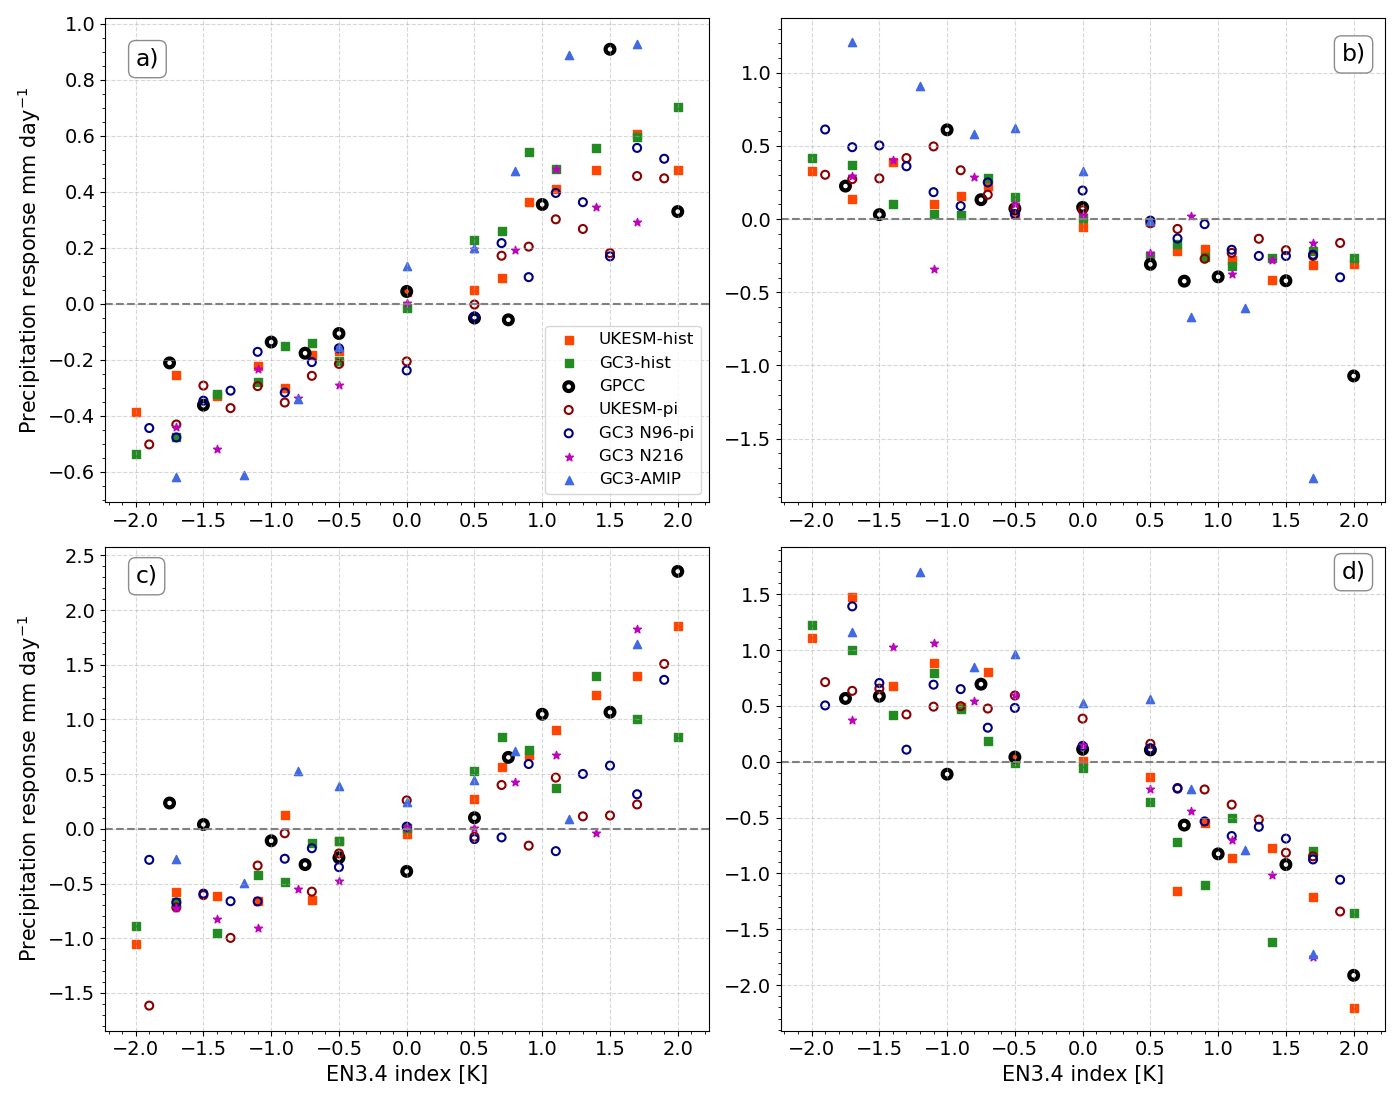
\includegraphics[width=\linewidth]{figures/fig_ensolinear}
\caption{ Precipitation response [mm day$^{-1}$] as a function of the El Ni\~no 3.4 index (see text) for (a) southwestern North America [20-37$^\circ$N, 112-98$^\circ$W], (b) Central America and southern Mexico [5-19$^\circ$N, 95-83$^\circ$W],, (c) South Eastern South America [35-25$^\circ$S, 60-50$^\circ$W], and (d) the Amazon [10-0$^\circ$S, 70-45$^\circ$W]. The observation scatter points are from GPCC in the period of 1940-2013.}
\label{fig:12}
\end{figure}

The climatological Walker circulation during DJF shows strong ascent in the 100-160$^\circ$E and the 280-310$^\circ$E regions, which correspond to the maritime continent and South America (Figure \ref{fig:swalker}a). During El Ni\~no events, there is increased specific humidity throughout the lower troposphere in the Central and Eastern Pacific, associated with ascending motions in this region and negative low-level wind anomalies and positive upper-level wind anomalies (Figure \ref{fig:swalker}d). In other words, an eastward shift of the Walker circulation. The wind, vertical velocity and specific humidity anomalies are the opposite during La Niña events, indicative of a stronger Walker circulation, slightly shifted to the west. 
The models seems to broadly reproduce the observed changes to the Walker circulation during ENSO events (Figure \ref{fig:swalker}).


% The strongest simulated response is that of GC3 N96-pi, especially over eastern Brazil and the equatorial Atlantic Ocean. 





 Figure \ref{fig:12} shows the observed and simulated precipitation responses in four regions of the AMS to different magnitudes of ENSO events, by binning events for their magnitude of the EN3.4 index and the corresponding precipitation anomaly from the climatology in each region. This figure aims to show  the degree of linearity of ENSO teleconnections to the AMS.
While the observed response shows some degree of linearity for El Ni\~no events in South America (panels c, d), the majority of the observed responses, particularly to La Ni\~na phases, are not linear.

 However, the simulations show several signs of linearity. For instance, consider the historical experiments, UKESM1-hist and GC3-hist, which show that the precipitation responses in southwestern North America, SESA and the Amazon increases roughly linearly as the magnitude of SST anomaly increases. In contrast, some other simulated responses, e.g. to La Ni\~na phases in South America in the piControl simulations, show signs of non-linearity.



\subsection{The role of ENSO flavours}
  
\begin{figure}[b!]
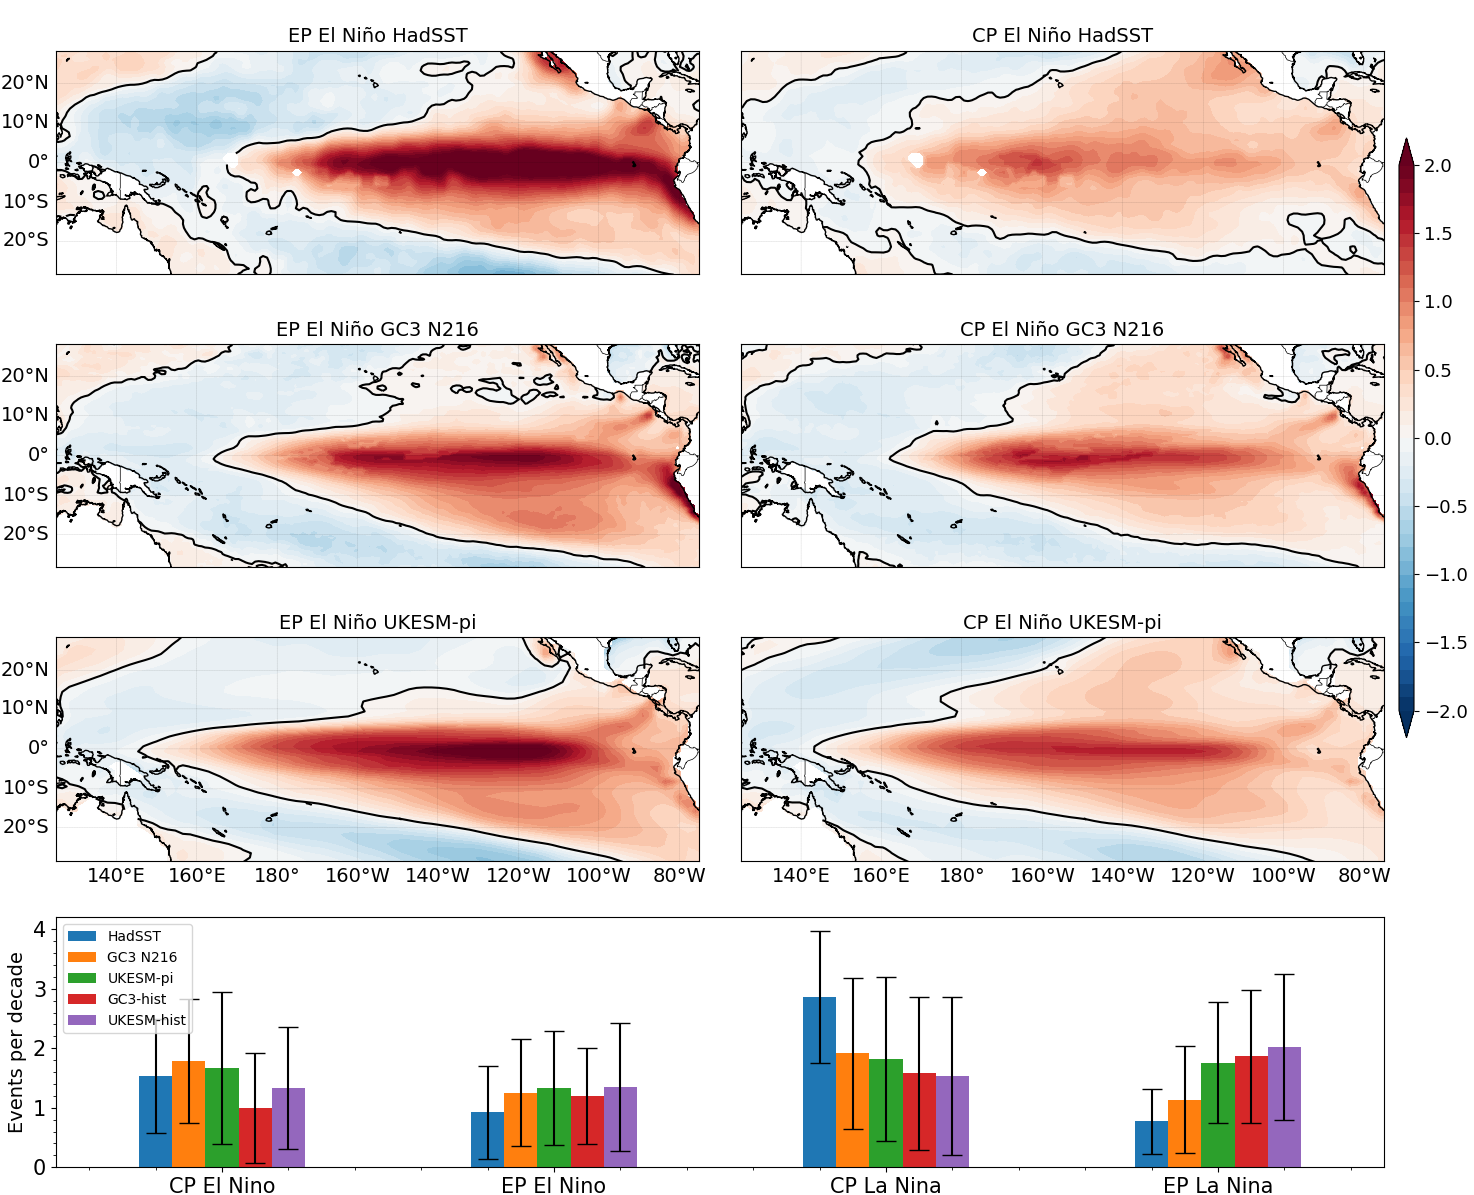
\includegraphics[width=\linewidth]{figures/epcpmap}
\caption{SST anomalies [K] for East Pacific (EP) and Central Pacific El Niño events in HadSST, GC3 N216 and UKESM piControl. EP (CP) events were defined where the E-index (C-index) was greater than 1. In the bottom panel, the frequency of events per decade (with standard deviation as error bar) is shown for HadSST and the simulations used in this study.
The E-index is computed from $(PC1-PC2)/\sqrt{2}$ and the C-index from $(PC1+PC2)/\sqrt(2)$.
}
\label{fig:s1}
\end{figure}


  
As described in section \ref{sub:lit_enso}, not all ENSO events are observed with the same SST anomaly pattern in the Pacific Ocean. These different SST patterns for each ENSO event are considered to be a source of non-linearity of ENSO impacts over South America \citep{sulca2018,cai2020}.
Principal component analysis has shown that ENSO events may be separated into two categories: Central Pacific (CP) and East Pacific (EP) events \citep{cai2020}, which highlight where the peak SST anomaly is found in the Pacific Ocean.
Figure \ref{fig:s1} shows that both UKESM1 and GC3 reasonably simulate the observed SST patterns associated with EP and CP El Niño events, although the simulations show CP SST patterns to spread further to the east than the HadSST dataset.
The simulations are also able to replicate very broadly the observed differences in the frequency of each event as CP La Niña events are more frequent than EP La Niña events, while the opposite is true for El Niño events.

\begin{figure}[t!]
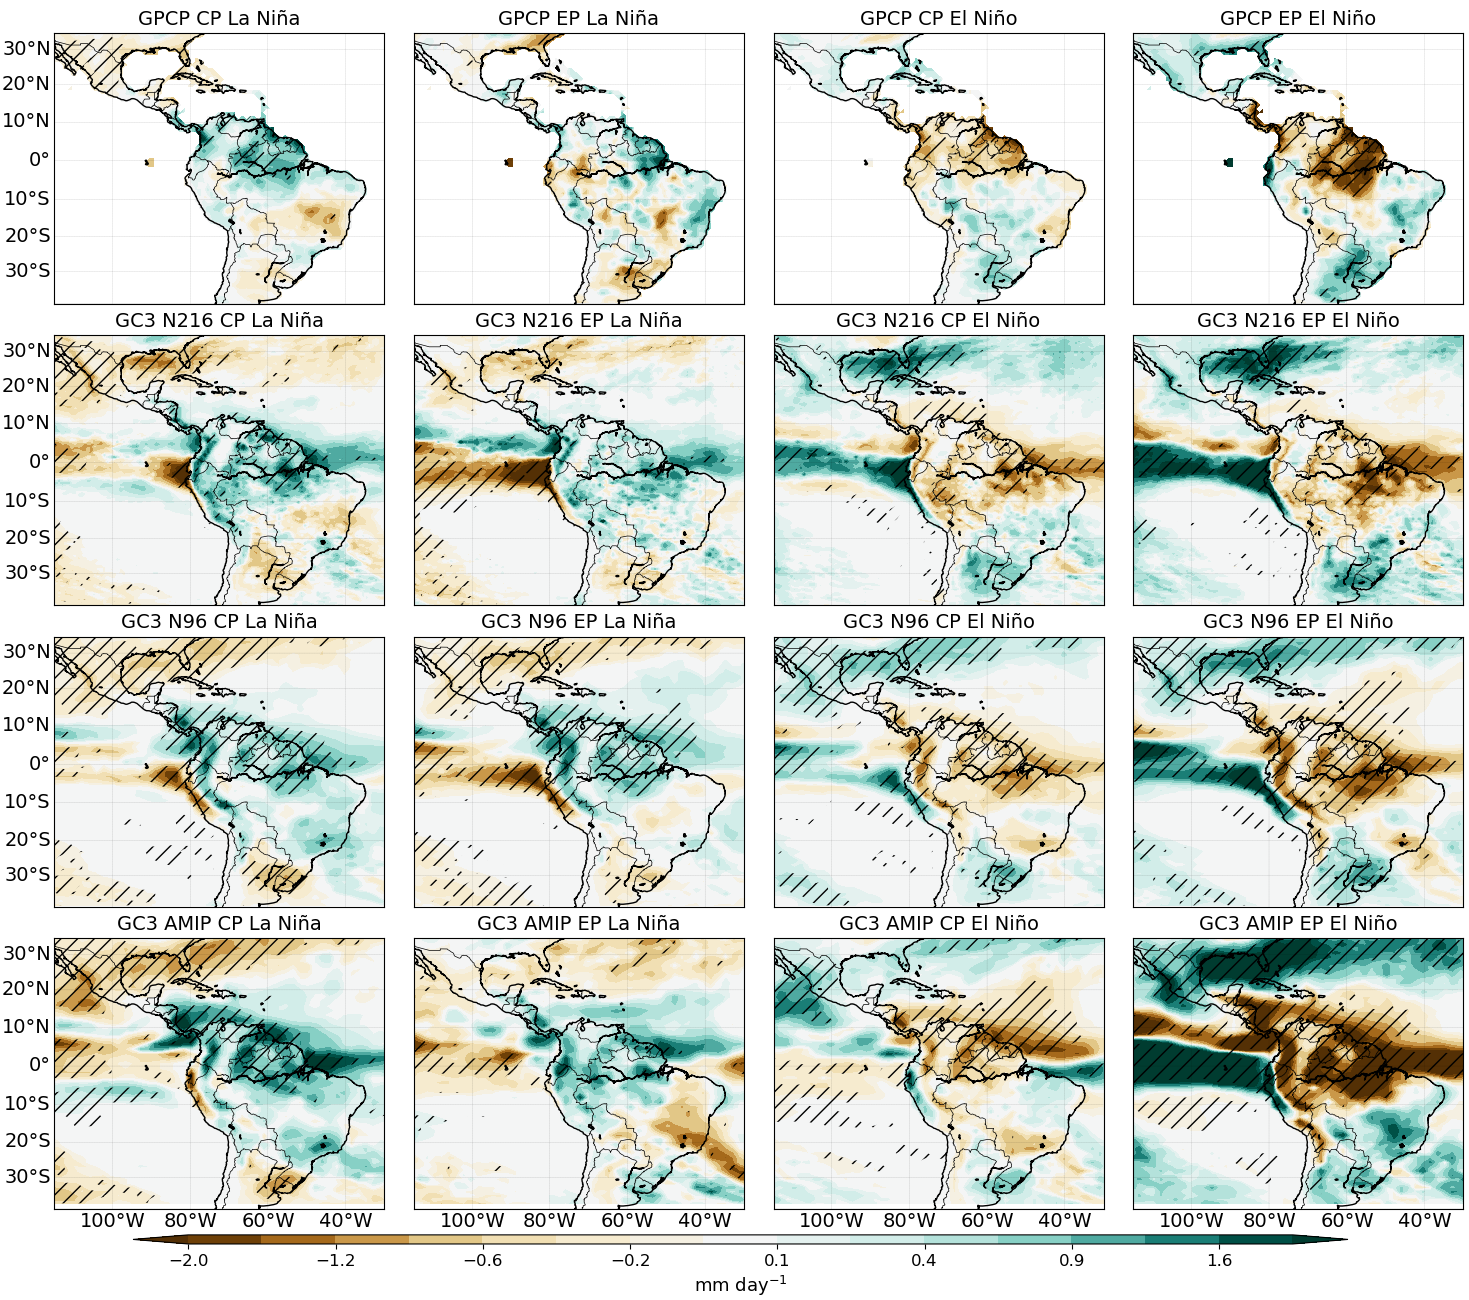
\includegraphics[width=\linewidth]{figures/cppranomalies_ff}
\caption{Precipitation anomalies in GPCC 1940-2013, GC3 N216-pi, GC3 N96-pi and GC3 AMIP for the four different types of ENSO events, as defined by \cite{cai2020}. Statistically significant anomalies (95\% confidence level) are hatched.}
\label{fig:senso}
\end{figure}  

Furthermore, Figure \ref{fig:senso} compares the precipitation anomalies for each type of ENSO event in observations with three simulations: GC3 N96-pi, GC3 N216-pi and GC3-amip. 
%The observations show significant precipitation responses differences in the Amazon, the Brazilian Nordeste and SESA between CP and EP events; however, these differences are less obvious in the coupled simulations (GC3 N96-pi, GC3 N216), but not in GC3 AMIP.
The observed precipitation response in the GPCC dataset to EP La Niña over equatorial South America is not significant and is smaller than the strong positive response to CP La Niña events in the same region. However,  the simulated response in GC3 N96-pi and GC3 N216 during La Niña events appears to be more independent of the type of event. In contrast, GC3-amip shows different magnitudes of responses to different types of La Niña events, in particular a positive, and significant, anomaly for CP La Niña events in the Amazon and weaker and not significant anomalies during EP events, which agrees with observations.

 The observed response to El Niño events in GPCC is also dependent on the type of event. EP EL Niño events show significant negative anomalies over the Amazon and positive anomalies over SESA whereas CP events only show significant anomalies (-1 mm day$^{-1}$) over northeastern South America. While the coupled models (GC3 N96-pi and GC3 N216) do show a stronger response to EP  EL Niño events than to CP events, the patterns of the response are very similar. In contrast, the response in GC3-amip agrees with observations. For this experiment, stronger negative responses to EP El Niño events are observed in the Amazon but the response to CP events is much weaker and is only significant in northeastern South America. In other words, GC3-amip agrees well with the observed non-linear teleconnection patterns whereas the  teleconnections in the coupled models do not depend  on the type of ENSO event.    

\subsection{A possible influence of the QBO on tropical ENSO teleconnections}

\begin{figure}[b!]
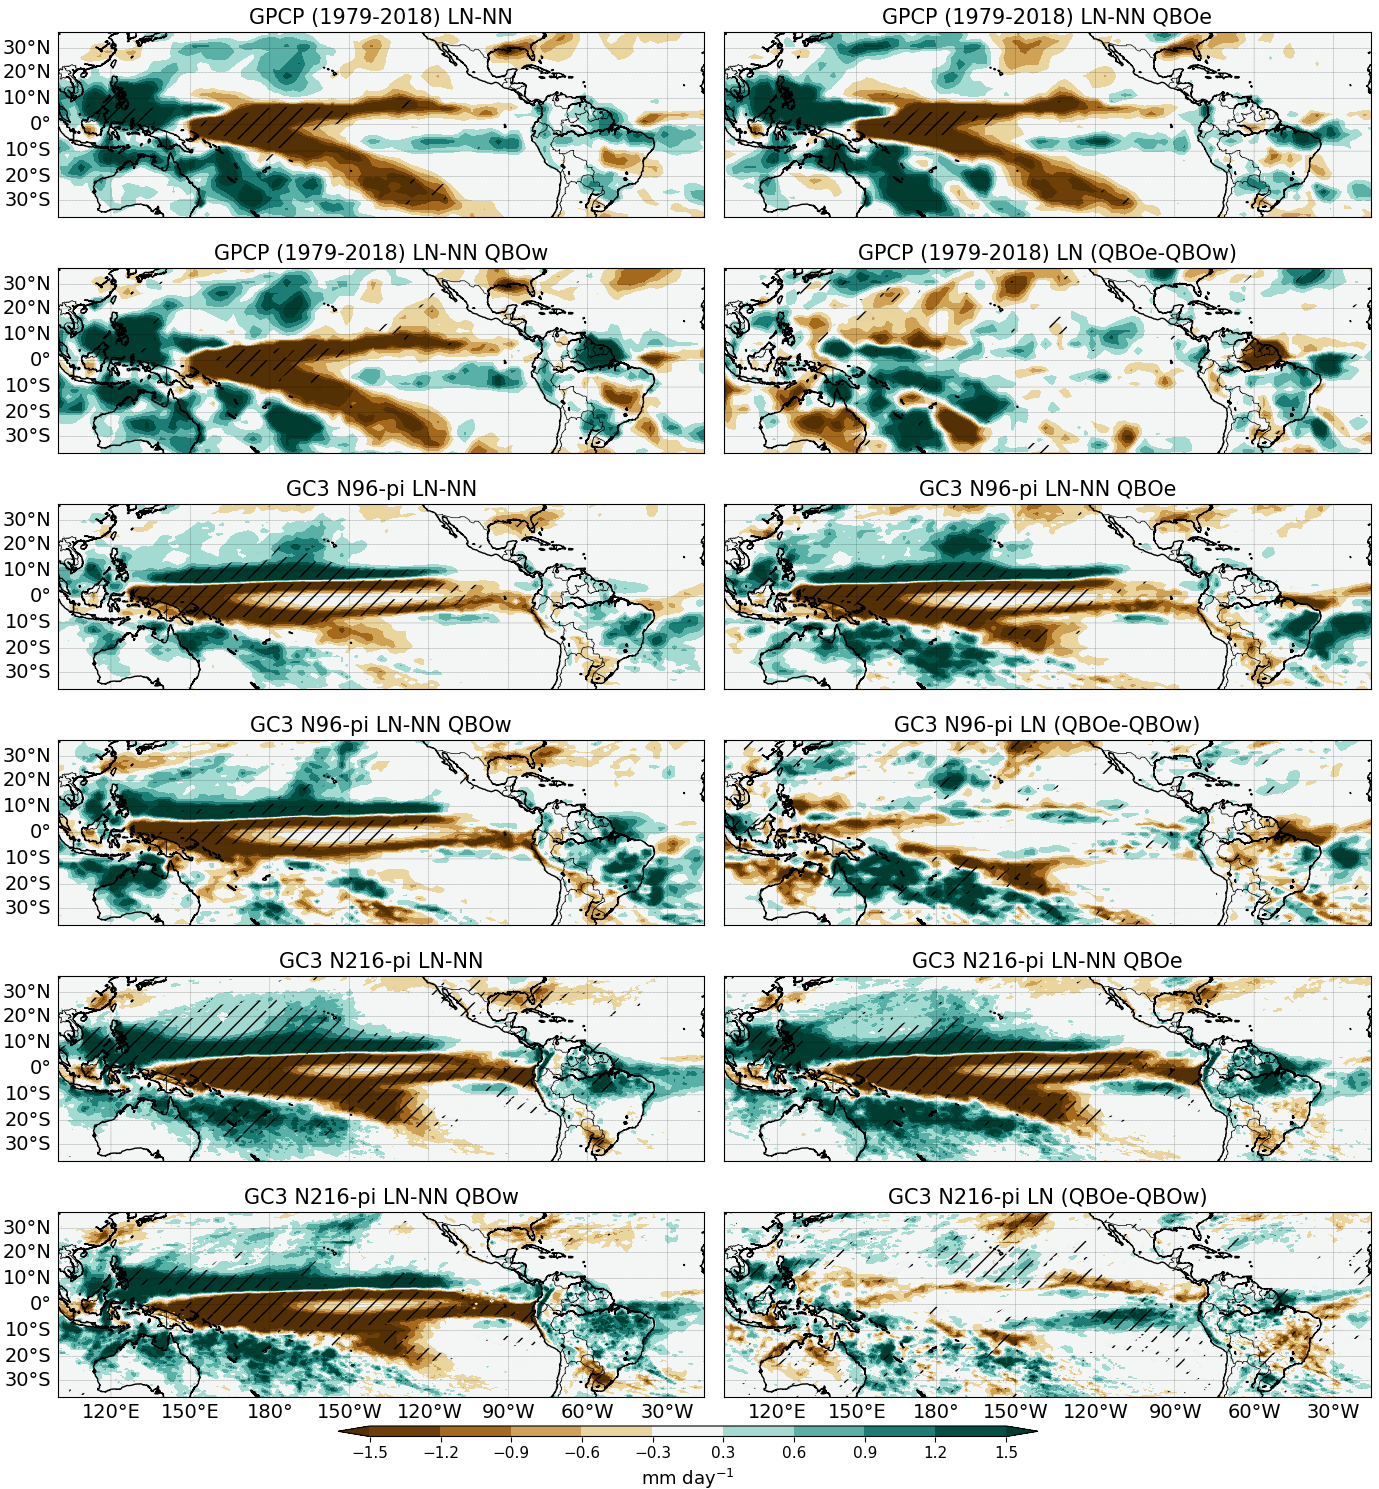
\includegraphics[width=\linewidth]{figures/trops_qbolnprfma}
\caption{Composite precipitation differences during JFMA in GPCP (1979-2018), GC3 N216-pi and GC3 N96-pi between (top) La Niña and Neutral ENSO conditions. The two middle panels show a subset of the top panel, by separating the La Niña composite based on the phase of the QBO. The lower panel shows the differences QBO E-W during La Niña periods. Statistically significant anomalies (95\% confidence level) are hatched.}
\label{fig:qbopr_pis}
\end{figure}  

Section \ref{sq:qbolit} discussed the observational and modelling evidence of the effects on deep convection associated with the stratospheric quasi-biennial oscillation (QBO). In particular, some evidence suggest that the QBO may play a role to determine interannual variability of the Walker circulation and monsoons \citep{giorgetta1999,collimore2003,liess2012}. 

This section evaluates whether the simulations analysed in this chapter, as well as observations, show signs of an influence of the QBO on the AMS. 
In particular, the analysis aims to understand whether the QBO may be a source of non-linearity and non-asymmetry for the teleconnections of ENSO associated with deep convection and the Walker circulation. In all cases, the phases of the QBO were defined using a 70 hPa zonal mean zonal wind index, with a threshold of +2 m s$^{-1}$ for the westerly phase (QBOw) and -2 m s$^{-1}$ for the easterly phase (QBOe).

Composites of the precipitation response to La Niña (LN) events in Figure \ref{fig:qbopr_pis} show that the phase of the QBO may be determine the strength and location of the teleconnection. 
While the precipitation difference in the western Pacific is relatively similar during QBOe than during QBOw in observations and simulations, the teleconnections to Australia, South America and the maritime continent are notably different depending on the QBO phase. 
In the GPCP dataset, the composite difference QBOe-QBOw during LN events suggests that the characteristic positive precipitation response during LN events in the Amazon, is largely associated with QBOw phases, whereas LN events during QBOe appear to have little effect over South America. 
A similar result is obtained for GC3 N96-pi. 


\begin{figure}[t!]
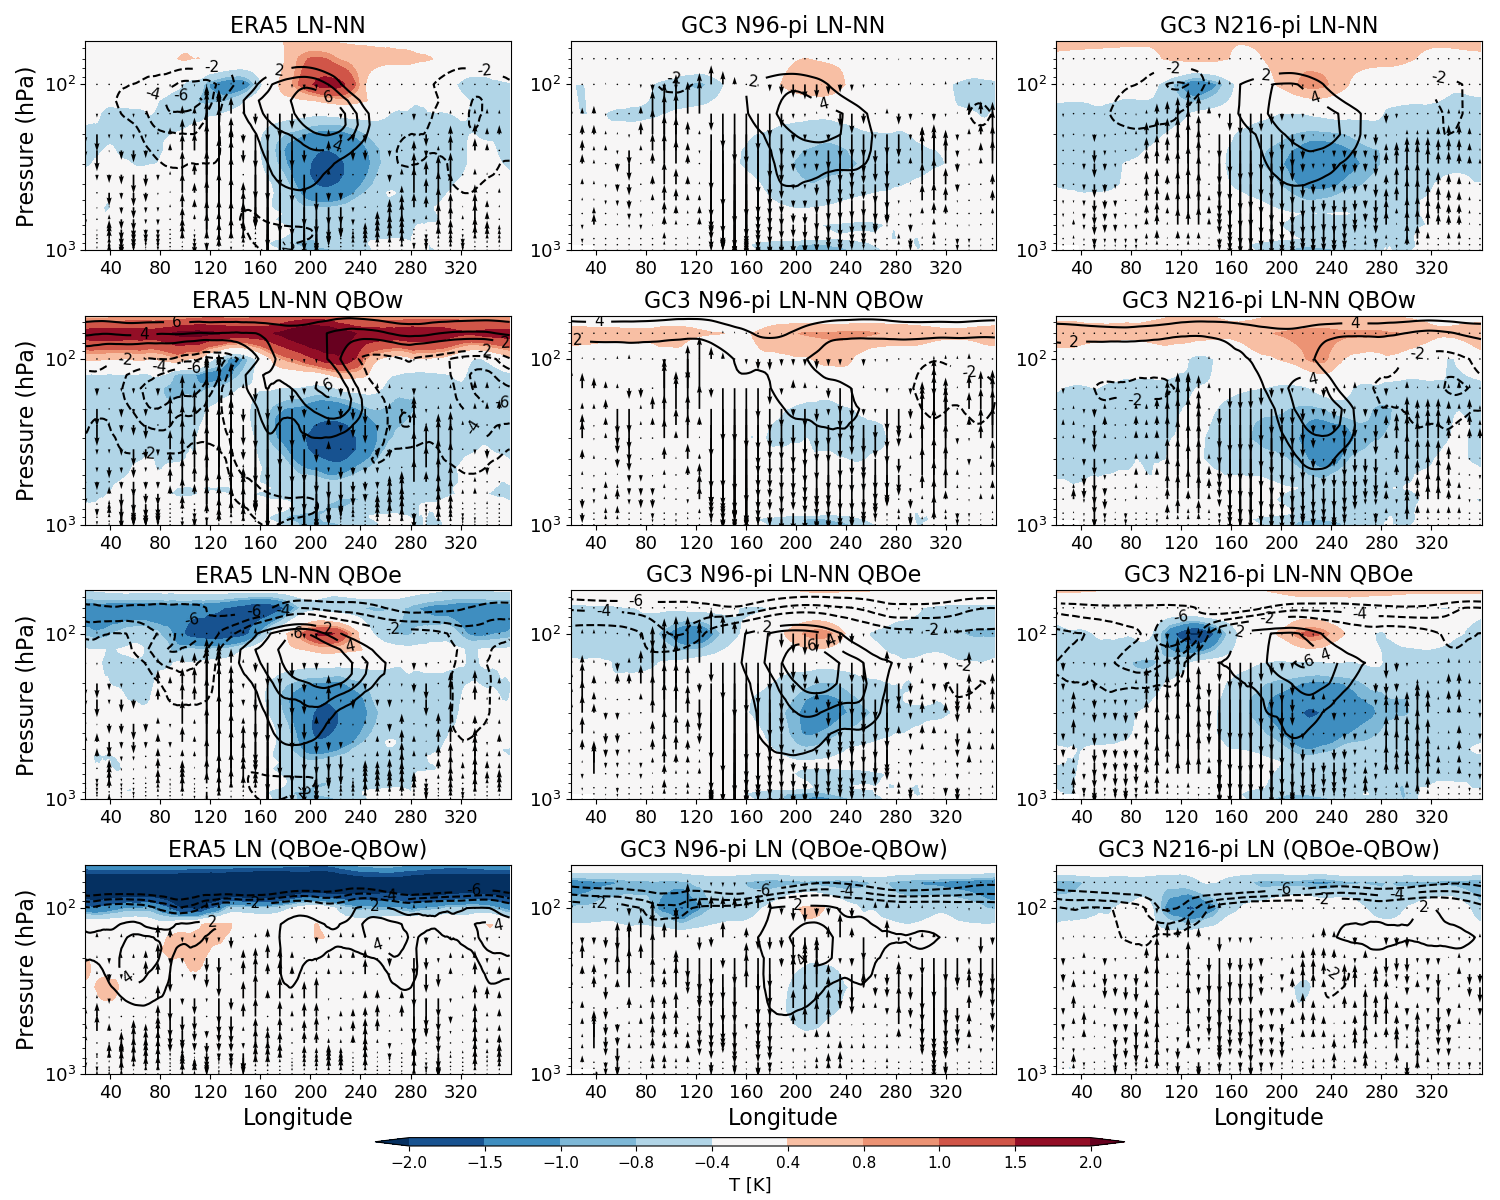
\includegraphics[width=\linewidth]{figures/walker_wqbo_jfma}
\caption{Longitude-height differences (JFMA) of equatorial (10S-10N) air temperature (color shading), zonal wind (contours) and vertical velocity ($\omega$ - vectors). The differences shown from top to bottom are between all La Niña (LN) periods and Neutral conditions (NN), between LN and NN during QBOw, LN-NN during QBOe, and the difference between LN events on different QBO phases (LN QBOe-QBOw). 
}
\label{fig:qbowalker_pis}
\end{figure}

These precipitation responses are further investigated by changes in the overturning circulation (Figure \ref{fig:qbowalker_pis}). As depicted in Figure \ref{fig:swalker}, La Niña events are associated with a westward shift in the Walker circulation with a strenghtening of the low-level easterlies in the Pacific Ocean. 
Figure \ref{fig:qbowalker_pis} shows that during LN the tropical troposphere cools and the UTLS region in the Central Pacific warms. These temperature anomalies are weaker in the simulations than in ERA5. 

The zonal wind anomalies in the upper-troposphere associated with LN events show different patterns and strengths during QBOw than during QBOe. The mean teleconnections during LN show positive upper-tropospheric anomalies above the Pacific Ocean,  but these anomalies are stronger during QBOe than during QBOw in ERA5 and the two simulations shown. In ERA5, most of the upper troposphere shows positive zonal wind differences in the QBOe-QBOw panel. 

There are three regions where ascending and descending motions are more greatly affected by LN events: the maritime continent, the Pacific Ocean and South America. The observed effect of the mean LN teleconnection is the following: anomalous ascent is seen in the maritime continent and in South America, in agreement with a stronger Walker circulation, whereas anomalous descending motions is observed in the Central and eastern Pacific associated with a westward shift of the Walker circulation. 


The effect of LN over ascending and descending motions is seemingly also affected by the QBO phase, according to the bottom panels of Figure \ref{fig:qbowalker_pis}. In ERA5 and the simulations, the anomalous ascent observed in South America during LN events is mostly associated with QBOw, whereas only small anomalous ascent is observed during QBOe. 
However, ERA5 disagrees with the simulations in the western Pacific region (140-180E), as the simulations suggest larger anomalous descent during QBOe than during QBOw, whereas in ERA5 these descending anomalies are larger during QBOw. 

A similar analysis was conducted to evaluate the effect of the QBO during the positive and the neutral phases of ENSO. These results are not shown because, although tentative suggestions were found that the QBO may play a role during these other phases of ENSO, there was little agreement between the models and ERA5/observations. Furthermore, the QBO representation in these CMIP6 models is biased in the UTLS region. In particular, the temperature signal associated with circulation of the QBO, most clearly seen in the bottom panels of Figure \ref{fig:qbowalker_pis}, is much weaker in the models. 

As suggested by the literature summarised in section \ref{sq:qbolit}, this temperature signal could be the key aspect of any effect of the QBO on deep convective systems, and as such, the evidence from a short record (ERA5) or models with key biases in possible processes involved presented in this chapter warrants both caution and more work. 
This topic will be investigated in the next chapters.

\section{Summary and discussion}



 This chapter assessed the MOHC models, HadGEM3 and UKESM1, in their pre-industrial control, historical and AMIP experiment contributions to CMIP6 with specific emphasis on the AMS and associated large-scale tropical circulation. The selected CMIP6 experiments allow to assess the effect of including Earth System processes or increasing resolution for representing regional monsoon rainfall. 
A schematic in Figure \ref{fig:13} shows the primary components of the AMS climate and summarises the main biases found in these simulations and this chapter.
%The study focuses on four regions in the AMS domain, the North American Monsoon, the MSD region of southern Mexico and Central America, southeastern Brazil and the Amazon.



Rainfall in the North American Monsoon was particularly well simulated by the models. The seasonal cycle, peak monsoon rainfall rates and timings of monsoon onset and retreat in the simulations agreed well with TRMM. The historical experiments overestimate the mean temperature in most of the Americas by 1.5 K, but particularly in boreal summer in southwestern North America (+4 K). In spite of this warm bias, the temperature seasonal cycle is well represented by these models. 

  These results suggest model improvement on the simulation of the North American Monsoon from previous versions of the MOHC models \citep{arritt2000}, and most of the model cohorts of CMIP3 and CMIP5 \citep{geil2013}. For example, most of CMIP5 models showed a very wet bias during monsoon maturity whereas rainfall during monsoon maturity in all the experiments of this chapter are within less than 1 mm day$^{-1}$ of observations, during the maturity stage. However, these models continue to show biases during monsoon retreat as rainfall does not decrease as sharply as in observations after mid-September, which suggests a continued bias in the winter-time precipitation associated with cold-fronts \citep{adams1997}. Further research into variability of the North American seasonality may be explored using these models given their skillfull representation fo the seasonal cycle.

\begin{figure}[t!]
\centering
 %\noindent
 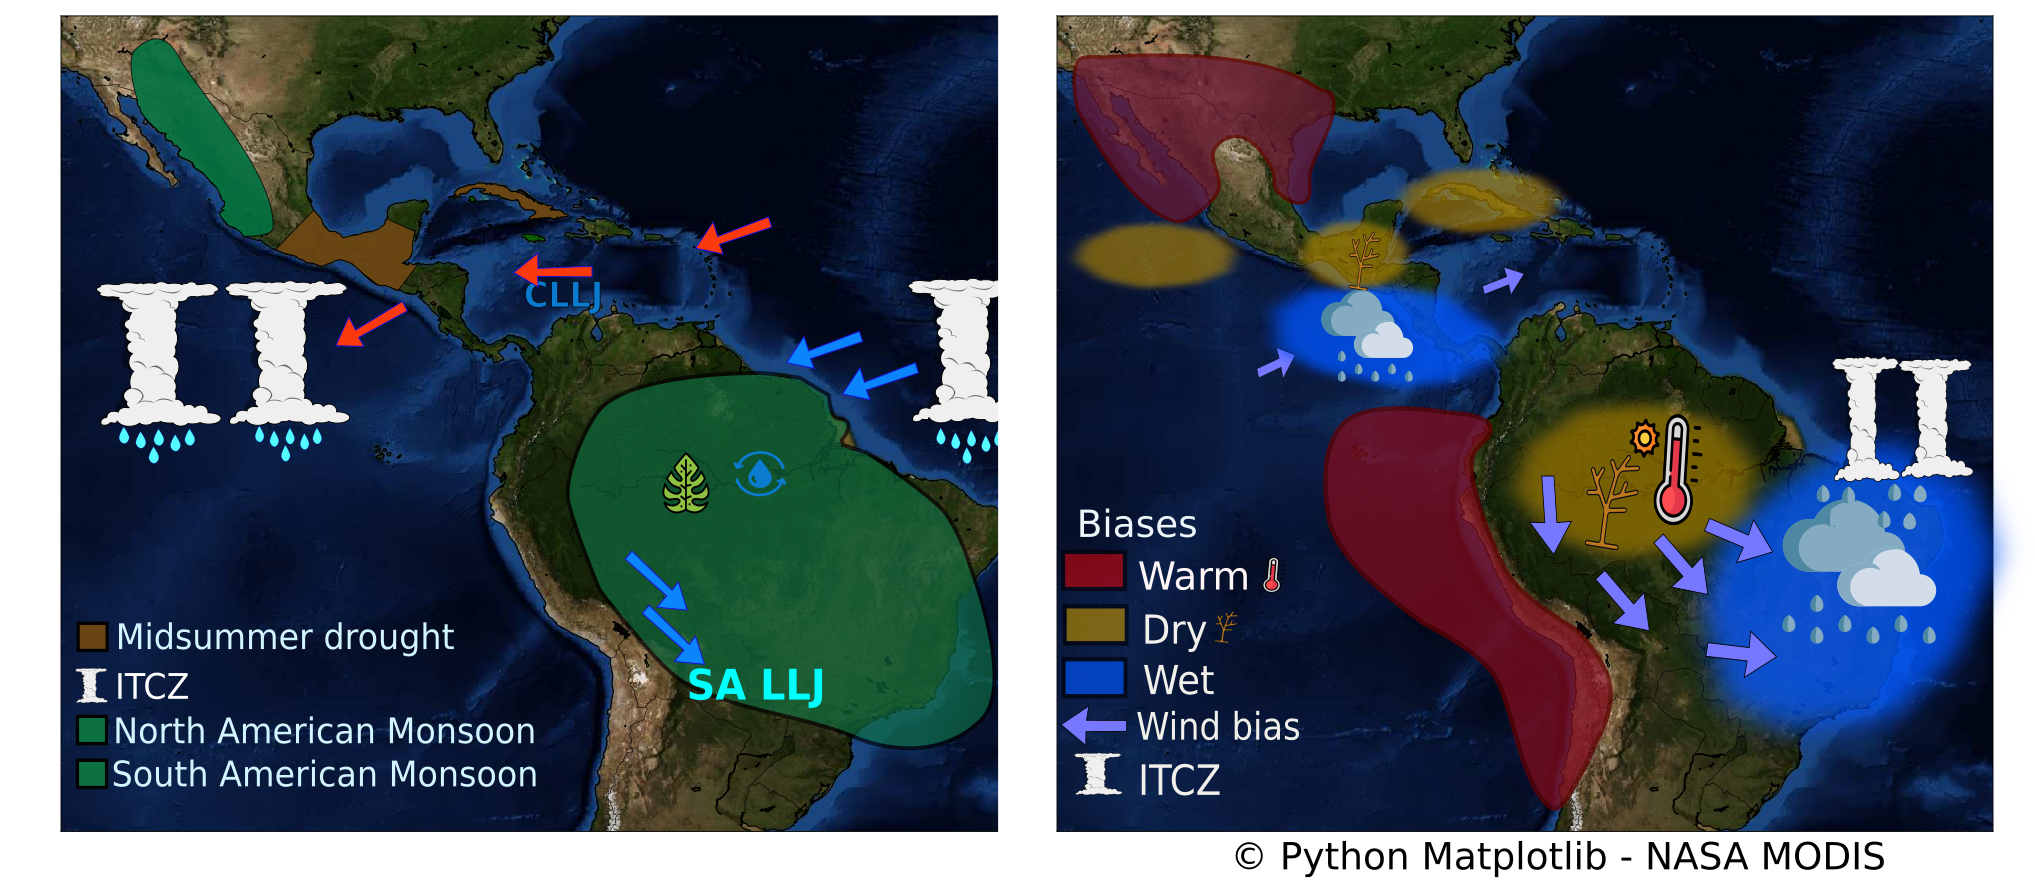
\includegraphics[width=\linewidth]{figures/drawing_d}
\caption{ Schematics of (a) the main features in the AMS and (b) the main biases in UKESM1 and HadGEM3. In (a) the boreal summer easterlies (red) and austral summer circulation (blue) are shown with the Caribbean and Bolivian Low-level Jets (CLLJ and BLLJ, respectively). In (b) the biases are shown for the respective northern and southern Hemisphere summers. The ITCZ bias in (b) refers to the southward displacement bias of the Atlantic ITCZ in the simulations.  }
\label{fig:13}
\end{figure}

    The Midsummer Drought (MSD) of southern Mexico and Central America is a regional feature of precipitation that most of CMIP5 models had difficulty capturing, with the MOHC models being amongst the few exceptions \citep{ryu2014}. 
The MSD in UKESM1 and GC3 continues to be relatively well represented; however, the experiments analysed in this chapter showed various  differences in the timing and strength of the bimodal cycle when compared to observed gridded-datasets and ERA5.  
%The MOHC models were amongst the minority of CMIP5 models that simulated a seasonal cycle with a two-peak structure separated by a drier period \citep{ryu2014}. 

The models simulate a wetter-than-observed first peak of precipitation and a drier MSD period, therefore simulating a larger difference between the first peak and the dry period. While in observations this difference  between the first peak and the MSD period ranges between 2-3 mm day$^{-1}$, in the simulations is difference is closer to 6 mm day$^{-1}$.
Rainfall during the first peak has been too wet in these models since CMIP3, suggesting a persistent wet bias in this region, likely associated with the bias in East Pacific ITCZ also shown in this chapter and in recent studies \citep{ryu2014,mulcahy2018}. 
In contrast, the so-called second peak of precipitation, observed in late August, is simulated in close agreement with TRMM, except in the AMIP experiment, which has a wet bias of 2 mm day$^{-1}$ at this stage.

The skill of UKESM1 and HadGEM to simulate the MSD's bimodal regime of precipitation makes these simulations ideal to understand the mechanisms underpinning the MSD and answer the question of why the MOHC do represent a MSD regime but other models fail. Furthermore, section \ref{sq:litmsd} discusses several open questions regarding the mechanisms that cause the observed MSD. These simulations will then be used in future chapters to address the evaluate previous hypotheses of the causes for the MSD. 


The East Pacific ITCZ migration and position was shown to be relatively well represented by the models (Figs. \ref{fig:3} and \ref{fig:4}). However, the models showed an overestimation of boreal summer rainfall near the coast of Central America (Figure \ref{fig:8}). These biases are associated with an easterly wind bias at low-levels, suggesting a bias in the flow from the Caribbean Sea into the Eastern Pacific  \citep{herrera2015,duranquesada2017}. 
The simulations also showed a biased Atlantic ITCZ that was displaced south of the observed ITCZ position during boreal winter (Figure \ref{fig:4}), particularly in the low resolution coupled simulations. 

In the Amazon, the simulations showed a warm bias (+2 K) during austral spring and summer, a bias that existed since CMIP5 \citep{jones2013}, and a colder than observed southeastern Brazil.
 These biases were linked with decreased cloud cover and less rainfall over the Amazon and more convective clouds and rainfall in southeastern Brazil (Figures \ref{fig:7} and \ref{fig:9}). 
The low cloud cover, warm and dry Amazon biases are intertwined with the low-level circulation from the Atlantic into the South American continent. The biases in the circulation during austral summer were observed as a northerly flow anomaly over the central and southern Amazon, a feature that has been associated with a stronger moisture transport away from the Amazon \citep{marengo2012,jones2017}. %The coupled simulations (Figure \ref{fig:7}) have a dry bias over the Amazon and a wet bias over southeastern Brazil. 


During the period of maximum rainfall rates in February, the simulations overestimate rainfall by 3 mm day$^{-1}$ in southeastern Brazil and underestimate rainfall in the Amazon by a similar rate. The historical experiments show a small drying response to historical forcing in the Amazon therefore slightly increasing the magnitude of this dry bias compared to the unforced piControl experiments.
The AMIP simulation with the SST biases removed improved the representation of the Atlantic ITCZ and the precipitation, cloud cover and temperature biases over the South American Monsoon.   The improvement in the circulation and precipitation biases in the AMIP simulation suggest that the origin of the dry Amazon bias are the biases in the Atlantic SSTs. 
%The simulated Amazon river basin also had shallower convection (higher 

  
The canonical teleconnection responses  of  temperature, SLP and precipitation in the AMS to ENSO events are well represented in these models. For example, the simulated spatial patterns and strength of the positive (negative) precipitation anomalies observed in northern Mexico and South Eastern South America during El Ni\~no (La Ni\~na) agree well with observations and reanalysis.
 Similarly, the teleconnection to the Amazon is well represented for both phases of ENSO, in spite of relevant biases in the mean state of the South American monsoon discussed above. %in the region.  
 
ENSO teleconnections in these simulations were found to be approximately linear, i.e., the precipitation response is linearly related to the magnitude of the SST perturbation in the EN 3.4 region. These experiments also show signs of symmetric teleconnections as positive and negative phases produce the opposite and equivalent precipitation response in the AMS. In contrast to observations and the GC3 AMIP simulation, the precipitation response in the coupled models appears to be independent of the type or flavour of ENSO events into Central and East Pacific events. The fact that these models show a reasonable representation of ENSO diversity in SST patterns but the models  do not replicate the observed non-linear dependance to ENSO events warrants further analysis.

The QBO appears to be a source of non-linearity for ENSO teleconnections to the Amazon. La Niña canonical teleconnections in the Amazon are characterized by a stronger ascent associated with a stronger Walker circulation. This teleconnection pattern occurs in observations and these simulations primarily during the westerly phase of the QBO, whereas the teleconnection during the easterly phase is much weaker and barely different from the climatological mean-state. Whether the stratospheric QBO poses such an important control to the main source of interannual variability for monsoon rainfall in the Amazon merits a separate chapter of this thesis. 

The main biases (Fig. \ref{fig:13}), in these experiments are generally smaller in the medium resolution GC3 N216 compared to the low resolution experiments, which suggests improved model performance with increased horizontal resolution.
In contrast, including Earth System processes in the UM model only affects the surface temperature response to historical forcing and not the dynamical biases that drive the precipitation and ITCZ biases. 

In short, the main dynamical biases in UKESM1 are very similar to those in GC3 N96 as these two models  share the same dynamical core; only when resolution is increased these biases are reduced notably. A noteworthy difference between UKESM1 and GC3 is that warming over the historical period in Mexico and the Amazon is higher in UKESM1 than in GC3. In general, UKESM1-hist shows a stronger temperature response to forcing than GC3-hist, as UKESM1 has been reported to have a  greater climate sensitivity than GC3 \citep{andrews2019,sellar2019}.  This differential warming may be a consequence of the land-use change in these regions playing a role in the UKESM1 representation of soil-atmosphere feedbacks. %In short, the main dynamical biases, such as the biased austral summer circulation in South America, are only improved when the resolution is increased, whereas the addition of Earth System processes does not improve dynamical biases that influence the characteristics of rainfall in the AMS. %This results suggets that improvement in monsoon representation is associated with resolution


%The results of this study showed that the medium resolution (GC3 N216) simulation improved upon some of the biases of the lower resolution simulations, such as most of the precipitation biases. %
The improvement in the medium resolution simulation compared to the low-resolution simulations may  be associated to the improved dynamics of the ocean or the atmosphere. %associated with relying less on model parametrisations.
For example, the Atlantic ITCZ biases have been shown to be directly affected by processes in the convective scheme \citep{bellucci2010}, such as the treatment of entrainment and moisture-cloud feedbacks \citep{oueslati2013,li2014}. 
The resolution of the ocean model has been shown to impact the eddy heat flux parametrisation and the associated heat uptake and transport of the ocean  \citep{kuhlbrodt2018}. The improvement in the Atlantic SSTs and ITCZ and the associated dynamics in GC3 N216-pi also improves the associated circulation biases and moisture transport in the South American Monsoon. In other words, the oceanic resolution may play an important role in the cross-equatorial heat and moisture transport, SST gradients over the equatorial Atlantic which in turns improves the land-sea circulation over the Amazon during austral summer, a circulation that is key for representing the spatial distribution of rainfall in South America.

%These CMIP6 simulations of HadGEM3 and UKESM1 show some signs of model improvement, particularly in the North American Monsoon and may be used to better understand the response to current and future response to anthropogenic forcing. Furthermore, several aspects of the climate of the AMS that are well simulated by these models, such as a good representation of the MSD and a resonable representation of ENSO diversity, may suggest further use of these simulations to address outstanding questions of climate variability in this region across different temporal scales.


